% Options for packages loaded elsewhere
\PassOptionsToPackage{unicode}{hyperref}
\PassOptionsToPackage{hyphens}{url}
\PassOptionsToPackage{dvipsnames,svgnames,x11names}{xcolor}
%
\documentclass[
]{article}
\usepackage{amsmath,amssymb}
\usepackage{lmodern}
\usepackage{iftex}
\ifPDFTeX
  \usepackage[T1]{fontenc}
  \usepackage[utf8]{inputenc}
  \usepackage{textcomp} % provide euro and other symbols
\else % if luatex or xetex
  \usepackage{unicode-math}
  \defaultfontfeatures{Scale=MatchLowercase}
  \defaultfontfeatures[\rmfamily]{Ligatures=TeX,Scale=1}
  \setmainfont[]{fouriernc}
\fi
% Use upquote if available, for straight quotes in verbatim environments
\IfFileExists{upquote.sty}{\usepackage{upquote}}{}
\IfFileExists{microtype.sty}{% use microtype if available
  \usepackage[]{microtype}
  \UseMicrotypeSet[protrusion]{basicmath} % disable protrusion for tt fonts
}{}
\makeatletter
\@ifundefined{KOMAClassName}{% if non-KOMA class
  \IfFileExists{parskip.sty}{%
    \usepackage{parskip}
  }{% else
    \setlength{\parindent}{0pt}
    \setlength{\parskip}{6pt plus 2pt minus 1pt}}
}{% if KOMA class
  \KOMAoptions{parskip=half}}
\makeatother
\usepackage{xcolor}
\usepackage[margin=1in]{geometry}
\usepackage{color}
\usepackage{fancyvrb}
\newcommand{\VerbBar}{|}
\newcommand{\VERB}{\Verb[commandchars=\\\{\}]}
\DefineVerbatimEnvironment{Highlighting}{Verbatim}{commandchars=\\\{\}}
% Add ',fontsize=\small' for more characters per line
\usepackage{framed}
\definecolor{shadecolor}{RGB}{248,248,248}
\newenvironment{Shaded}{\begin{snugshade}}{\end{snugshade}}
\newcommand{\AlertTok}[1]{\textcolor[rgb]{0.94,0.16,0.16}{#1}}
\newcommand{\AnnotationTok}[1]{\textcolor[rgb]{0.56,0.35,0.01}{\textbf{\textit{#1}}}}
\newcommand{\AttributeTok}[1]{\textcolor[rgb]{0.77,0.63,0.00}{#1}}
\newcommand{\BaseNTok}[1]{\textcolor[rgb]{0.00,0.00,0.81}{#1}}
\newcommand{\BuiltInTok}[1]{#1}
\newcommand{\CharTok}[1]{\textcolor[rgb]{0.31,0.60,0.02}{#1}}
\newcommand{\CommentTok}[1]{\textcolor[rgb]{0.56,0.35,0.01}{\textit{#1}}}
\newcommand{\CommentVarTok}[1]{\textcolor[rgb]{0.56,0.35,0.01}{\textbf{\textit{#1}}}}
\newcommand{\ConstantTok}[1]{\textcolor[rgb]{0.00,0.00,0.00}{#1}}
\newcommand{\ControlFlowTok}[1]{\textcolor[rgb]{0.13,0.29,0.53}{\textbf{#1}}}
\newcommand{\DataTypeTok}[1]{\textcolor[rgb]{0.13,0.29,0.53}{#1}}
\newcommand{\DecValTok}[1]{\textcolor[rgb]{0.00,0.00,0.81}{#1}}
\newcommand{\DocumentationTok}[1]{\textcolor[rgb]{0.56,0.35,0.01}{\textbf{\textit{#1}}}}
\newcommand{\ErrorTok}[1]{\textcolor[rgb]{0.64,0.00,0.00}{\textbf{#1}}}
\newcommand{\ExtensionTok}[1]{#1}
\newcommand{\FloatTok}[1]{\textcolor[rgb]{0.00,0.00,0.81}{#1}}
\newcommand{\FunctionTok}[1]{\textcolor[rgb]{0.00,0.00,0.00}{#1}}
\newcommand{\ImportTok}[1]{#1}
\newcommand{\InformationTok}[1]{\textcolor[rgb]{0.56,0.35,0.01}{\textbf{\textit{#1}}}}
\newcommand{\KeywordTok}[1]{\textcolor[rgb]{0.13,0.29,0.53}{\textbf{#1}}}
\newcommand{\NormalTok}[1]{#1}
\newcommand{\OperatorTok}[1]{\textcolor[rgb]{0.81,0.36,0.00}{\textbf{#1}}}
\newcommand{\OtherTok}[1]{\textcolor[rgb]{0.56,0.35,0.01}{#1}}
\newcommand{\PreprocessorTok}[1]{\textcolor[rgb]{0.56,0.35,0.01}{\textit{#1}}}
\newcommand{\RegionMarkerTok}[1]{#1}
\newcommand{\SpecialCharTok}[1]{\textcolor[rgb]{0.00,0.00,0.00}{#1}}
\newcommand{\SpecialStringTok}[1]{\textcolor[rgb]{0.31,0.60,0.02}{#1}}
\newcommand{\StringTok}[1]{\textcolor[rgb]{0.31,0.60,0.02}{#1}}
\newcommand{\VariableTok}[1]{\textcolor[rgb]{0.00,0.00,0.00}{#1}}
\newcommand{\VerbatimStringTok}[1]{\textcolor[rgb]{0.31,0.60,0.02}{#1}}
\newcommand{\WarningTok}[1]{\textcolor[rgb]{0.56,0.35,0.01}{\textbf{\textit{#1}}}}
\usepackage{graphicx}
\makeatletter
\def\maxwidth{\ifdim\Gin@nat@width>\linewidth\linewidth\else\Gin@nat@width\fi}
\def\maxheight{\ifdim\Gin@nat@height>\textheight\textheight\else\Gin@nat@height\fi}
\makeatother
% Scale images if necessary, so that they will not overflow the page
% margins by default, and it is still possible to overwrite the defaults
% using explicit options in \includegraphics[width, height, ...]{}
\setkeys{Gin}{width=\maxwidth,height=\maxheight,keepaspectratio}
% Set default figure placement to htbp
\makeatletter
\def\fps@figure{htbp}
\makeatother
\setlength{\emergencystretch}{3em} % prevent overfull lines
\providecommand{\tightlist}{%
  \setlength{\itemsep}{0pt}\setlength{\parskip}{0pt}}
\setcounter{secnumdepth}{-\maxdimen} % remove section numbering
\newcommand{\indep}{\perp \!\!\! \perp}
\usepackage[T1]{fontenc}
\usepackage{fouriernc}
\usepackage{setspace}\onehalfspacing
\usepackage{amsfonts}
\usepackage{dcolumn}
\usepackage{pifont}
\usepackage{booktabs}
\usepackage{placeins}
\usepackage{booktabs}
\usepackage{siunitx}

  \newcolumntype{d}{S[
    input-open-uncertainty=,
    input-close-uncertainty=,
    parse-numbers = false,
    table-align-text-pre=false,
    table-align-text-post=false
  ]}
  
\usepackage{longtable}
\usepackage{array}
\usepackage{multirow}
\usepackage{wrapfig}
\usepackage{float}
\usepackage{colortbl}
\usepackage{pdflscape}
\usepackage{tabu}
\usepackage{threeparttable}
\usepackage{threeparttablex}
\usepackage[normalem]{ulem}
\usepackage{makecell}
\usepackage{xcolor}
\ifLuaTeX
  \usepackage{selnolig}  % disable illegal ligatures
\fi
\IfFileExists{bookmark.sty}{\usepackage{bookmark}}{\usepackage{hyperref}}
\IfFileExists{xurl.sty}{\usepackage{xurl}}{} % add URL line breaks if available
\urlstyle{same} % disable monospaced font for URLs
\hypersetup{
  pdftitle={Did political trust moderate the relationship between economic insecurity and AfD voting in the 2021 extit\{Bundestagswahl\}?},
  pdfauthor={Jacob Edenhofer},
  colorlinks=true,
  linkcolor={cyan},
  filecolor={Maroon},
  citecolor={Blue},
  urlcolor={magenta},
  pdfcreator={LaTeX via pandoc}}

\title{Did political trust moderate the relationship between economic
insecurity and AfD voting in the 2021 extit\{Bundestagswahl\}?}
\usepackage{etoolbox}
\makeatletter
\providecommand{\subtitle}[1]{% add subtitle to \maketitle
  \apptocmd{\@title}{\par {\large #1 \par}}{}{}
}
\makeatother
\subtitle{Final AVCD assignment}
\author{Jacob Edenhofer\footnote{\href{mailto:jacob.edenhofer@some.ox.ac.uk}{\nolinkurl{jacob.edenhofer@some.ox.ac.uk}}}}
\date{20 May 2023}

\begin{document}
\maketitle

\hypertarget{preliminaries}{%
\section{Preliminaries}\label{preliminaries}}

\begin{Shaded}
\begin{Highlighting}[]
\CommentTok{\# load relevant packages }
\FunctionTok{library}\NormalTok{(tidyverse)}
\FunctionTok{library}\NormalTok{(haven)}
\FunctionTok{library}\NormalTok{(modelsummary)}
\FunctionTok{library}\NormalTok{(survey)}
\FunctionTok{library}\NormalTok{(here)}
\FunctionTok{library}\NormalTok{(ggeffects)}
\FunctionTok{library}\NormalTok{(margins)}

\CommentTok{\# import data }
\NormalTok{gles }\OtherTok{\textless{}{-}} \FunctionTok{read\_dta}\NormalTok{(}\FunctionTok{paste0}\NormalTok{(}\FunctionTok{here}\NormalTok{(), }\StringTok{"/Data/german\_longitudinal\_election\_study\_cross\_section\_post\_election2021.dta"}\NormalTok{))}
\NormalTok{gles1 }\OtherTok{\textless{}{-}} \FunctionTok{read\_dta}\NormalTok{(}\FunctionTok{paste0}\NormalTok{(}\FunctionTok{here}\NormalTok{(), }\StringTok{"/Data/gles\_panel\_wave20.dta"}\NormalTok{))}
\end{Highlighting}
\end{Shaded}

Next, we will create some new variables:

\begin{Shaded}
\begin{Highlighting}[]
\NormalTok{gles\_mod }\OtherTok{\textless{}{-}}\NormalTok{ gles }\SpecialCharTok{\%\textgreater{}\%} 
  \FunctionTok{select}\NormalTok{(}\DecValTok{1}\SpecialCharTok{:}\DecValTok{100}\NormalTok{, }\FunctionTok{grep}\NormalTok{(}\StringTok{"d38|d4|q18|d63|d18|q63|d17|d8|d7|wum6|q13|q14|q15|q16|q18|q23|q24|q25|q26||q27q35|q37|q46|q78|q79|q125|q143"}\NormalTok{, }\FunctionTok{names}\NormalTok{(gles))) }\SpecialCharTok{\%\textgreater{}\%}
  \FunctionTok{mutate}\NormalTok{(}\AttributeTok{btw17\_zweitstimme =} \FunctionTok{ifelse}\NormalTok{(q34ba }\SpecialCharTok{\textless{}} \DecValTok{0}\NormalTok{, }\ConstantTok{NA}\NormalTok{, q34ba),}
         \AttributeTok{btw21\_zweitstimme =} \FunctionTok{ifelse}\NormalTok{(q114ba }\SpecialCharTok{\textless{}} \DecValTok{0}\NormalTok{, }\ConstantTok{NA}\NormalTok{, q114ba),}
         \AttributeTok{btw21\_turnout =} \FunctionTok{ifelse}\NormalTok{(q111 }\SpecialCharTok{\textless{}} \DecValTok{0} \SpecialCharTok{|}\NormalTok{ q111 }\SpecialCharTok{==} \DecValTok{8}\NormalTok{, }\ConstantTok{NA}\NormalTok{, q111),}
         \AttributeTok{btw21\_turnout1 =} \FunctionTok{ifelse}\NormalTok{(btw21\_turnout }\SpecialCharTok{==} \DecValTok{1}\NormalTok{, }\DecValTok{1}\NormalTok{, }\DecValTok{0}\NormalTok{),}
         \AttributeTok{year\_born =} \FunctionTok{ifelse}\NormalTok{(}\FunctionTok{grepl}\NormalTok{(}\StringTok{"{-}99|frueher"}\NormalTok{, d2a), }\ConstantTok{NA}\NormalTok{, d2a),}
         \AttributeTok{ostwest2\_dummy =} \FunctionTok{ifelse}\NormalTok{(ostwest2 }\SpecialCharTok{\textless{}} \DecValTok{0}\NormalTok{, }\ConstantTok{NA}\NormalTok{, ostwest2),}
         \AttributeTok{ostwest\_factor =} \FunctionTok{factor}\NormalTok{(ostwest2\_dummy, }
                                 \AttributeTok{levels =} \FunctionTok{c}\NormalTok{(}\DecValTok{0}\NormalTok{, }\DecValTok{1}\NormalTok{), }
                                 \AttributeTok{labels =} \FunctionTok{c}\NormalTok{(}\StringTok{"ost"}\NormalTok{, }\StringTok{"west"}\NormalTok{)),}
         \AttributeTok{sex =} \FunctionTok{ifelse}\NormalTok{(d1 }\SpecialCharTok{\textless{}} \DecValTok{0}\NormalTok{, }\ConstantTok{NA}\NormalTok{, d1),}
         \AttributeTok{sex1 =} \FunctionTok{factor}\NormalTok{(sex, }
                       \AttributeTok{levels =} \FunctionTok{c}\NormalTok{(}\DecValTok{1}\NormalTok{, }\DecValTok{2}\NormalTok{), }
                       \AttributeTok{labels =} \FunctionTok{c}\NormalTok{(}\StringTok{"male"}\NormalTok{, }\StringTok{"female"}\NormalTok{)),}
         \AttributeTok{year\_born1 =} \FunctionTok{as.numeric}\NormalTok{(}\FunctionTok{as.character}\NormalTok{(year\_born)),}
         \AttributeTok{age =} \DecValTok{2021} \SpecialCharTok{{-}} \FunctionTok{as.numeric}\NormalTok{(}\FunctionTok{as.character}\NormalTok{(year\_born)),}
         \AttributeTok{spd\_21 =} \FunctionTok{ifelse}\NormalTok{(btw21\_zweitstimme }\SpecialCharTok{==} \DecValTok{4}\NormalTok{, }\DecValTok{1}\NormalTok{, }\DecValTok{0}\NormalTok{),}
         \AttributeTok{union\_21 =} \FunctionTok{ifelse}\NormalTok{(btw21\_zweitstimme }\SpecialCharTok{==} \DecValTok{1}\NormalTok{, }\DecValTok{1}\NormalTok{, }\DecValTok{0}\NormalTok{),}
         \AttributeTok{gruene\_21 =} \FunctionTok{ifelse}\NormalTok{(btw21\_zweitstimme }\SpecialCharTok{==} \DecValTok{6}\NormalTok{, }\DecValTok{1}\NormalTok{, }\DecValTok{0}\NormalTok{),}
         \AttributeTok{fdp\_21 =} \FunctionTok{ifelse}\NormalTok{(btw21\_zweitstimme }\SpecialCharTok{==} \DecValTok{5}\NormalTok{, }\DecValTok{1}\NormalTok{, }\DecValTok{0}\NormalTok{),}
         \AttributeTok{afd\_21 =} \FunctionTok{ifelse}\NormalTok{(btw21\_zweitstimme }\SpecialCharTok{==} \DecValTok{322}\NormalTok{, }\DecValTok{1}\NormalTok{, }\DecValTok{0}\NormalTok{),}
         \AttributeTok{linke\_21 =} \FunctionTok{ifelse}\NormalTok{(btw21\_zweitstimme }\SpecialCharTok{==} \DecValTok{7}\NormalTok{, }\DecValTok{1}\NormalTok{, }\DecValTok{0}\NormalTok{), }
         \AttributeTok{spd\_to\_switch =} \FunctionTok{ifelse}\NormalTok{(btw21\_zweitstimme }\SpecialCharTok{==} \DecValTok{4} \SpecialCharTok{\&}\NormalTok{ btw17\_zweitstimme }\SpecialCharTok{!=} \DecValTok{4}\NormalTok{, }\DecValTok{1}\NormalTok{, }\DecValTok{0}\NormalTok{),}
         \AttributeTok{afd\_away\_switch =} \FunctionTok{ifelse}\NormalTok{(btw17\_zweitstimme }\SpecialCharTok{==} \DecValTok{322} \SpecialCharTok{\&}\NormalTok{ btw21\_zweitstimme }\SpecialCharTok{!=} \DecValTok{322}\NormalTok{, }\DecValTok{1}\NormalTok{, }\DecValTok{0}\NormalTok{),}
         \AttributeTok{constituency\_centric\_rep =} \FunctionTok{ifelse}\NormalTok{(q63a }\SpecialCharTok{\textless{}} \DecValTok{0}\NormalTok{, }\ConstantTok{NA}\NormalTok{, q63a),}
         \AttributeTok{party\_centric\_rep =} \FunctionTok{ifelse}\NormalTok{(q63c }\SpecialCharTok{\textless{}} \DecValTok{0}\NormalTok{, }\ConstantTok{NA}\NormalTok{, q63c),}
         \AttributeTok{household\_income =} \FunctionTok{ifelse}\NormalTok{(d63 }\SpecialCharTok{\textless{}} \DecValTok{0}\NormalTok{, }\ConstantTok{NA}\NormalTok{, d63),}
         \AttributeTok{household\_income\_factor =} \FunctionTok{as.factor}\NormalTok{(household\_income),}
         \AttributeTok{bachelor\_dummy =} \FunctionTok{ifelse}\NormalTok{(d8j1 }\SpecialCharTok{\textless{}} \DecValTok{0}\NormalTok{, }\ConstantTok{NA}\NormalTok{, d8j1),}
         \AttributeTok{school =} \FunctionTok{ifelse}\NormalTok{(d7 }\SpecialCharTok{\textless{}} \DecValTok{0}\NormalTok{, }\ConstantTok{NA}\NormalTok{, d7),}
         \AttributeTok{abitur =} \FunctionTok{ifelse}\NormalTok{(d7 }\SpecialCharTok{==} \DecValTok{5}\NormalTok{, }\DecValTok{1}\NormalTok{, }\DecValTok{0}\NormalTok{),}
         \AttributeTok{abitur\_factor =} \FunctionTok{ifelse}\NormalTok{(abitur }\SpecialCharTok{==} \DecValTok{1}\NormalTok{, }\StringTok{"abitur"}\NormalTok{, }\StringTok{"no\_abitur"}\NormalTok{),}
         \AttributeTok{urban\_rural =} \FunctionTok{ifelse}\NormalTok{(wum6 }\SpecialCharTok{\textless{}} \DecValTok{0}\NormalTok{, }\ConstantTok{NA}\NormalTok{, wum6),}
         \AttributeTok{urban\_rural\_factor =} \FunctionTok{as.factor}\NormalTok{(urban\_rural),}
         \AttributeTok{subjective\_class =} \FunctionTok{ifelse}\NormalTok{(d38 }\SpecialCharTok{\textless{}} \DecValTok{0}\NormalTok{, }\ConstantTok{NA}\NormalTok{, d38),}
         \AttributeTok{left\_right\_self =} \FunctionTok{ifelse}\NormalTok{(q37 }\SpecialCharTok{\textless{}} \DecValTok{0}\NormalTok{, }\ConstantTok{NA}\NormalTok{, q37),}
         \AttributeTok{left\_right\_self\_factor =} \FunctionTok{as.factor}\NormalTok{(left\_right\_self),}
         \AttributeTok{left\_right\_cdu =} \FunctionTok{ifelse}\NormalTok{(q35b }\SpecialCharTok{\textless{}} \DecValTok{0}\NormalTok{, }\ConstantTok{NA}\NormalTok{, q35b),}
         \AttributeTok{left\_right\_cdu\_factor =} \FunctionTok{as.factor}\NormalTok{(left\_right\_cdu),}
         \AttributeTok{distance\_cdu =}\NormalTok{ (left\_right\_cdu}\SpecialCharTok{{-}}\NormalTok{left\_right\_self)}\SpecialCharTok{\^{}}\DecValTok{2}\NormalTok{,}
         \AttributeTok{left\_right\_csu =} \FunctionTok{ifelse}\NormalTok{(q35c }\SpecialCharTok{\textless{}} \DecValTok{0}\NormalTok{, }\ConstantTok{NA}\NormalTok{, q35c),}
         \AttributeTok{left\_right\_csu\_factor =} \FunctionTok{as.factor}\NormalTok{(left\_right\_csu),}
         \AttributeTok{distance\_csu =}\NormalTok{ (left\_right\_csu}\SpecialCharTok{{-}}\NormalTok{left\_right\_self)}\SpecialCharTok{\^{}}\DecValTok{2}\NormalTok{,}
         \AttributeTok{left\_right\_spd =} \FunctionTok{ifelse}\NormalTok{(q35d }\SpecialCharTok{\textless{}} \DecValTok{0}\NormalTok{, }\ConstantTok{NA}\NormalTok{, q35d),}
         \AttributeTok{left\_right\_spd\_factor =} \FunctionTok{as.factor}\NormalTok{(left\_right\_spd),}
         \AttributeTok{distance\_spd =}\NormalTok{ (left\_right\_spd}\SpecialCharTok{{-}}\NormalTok{left\_right\_self)}\SpecialCharTok{\^{}}\DecValTok{2}\NormalTok{,}
         \AttributeTok{left\_right\_afd =} \FunctionTok{ifelse}\NormalTok{(q35h }\SpecialCharTok{\textless{}} \DecValTok{0}\NormalTok{, }\ConstantTok{NA}\NormalTok{, q35h),}
         \AttributeTok{left\_right\_afd\_factor =} \FunctionTok{as.factor}\NormalTok{(left\_right\_afd),}
         \AttributeTok{distance\_afd =}\NormalTok{ (left\_right\_afd}\SpecialCharTok{{-}}\NormalTok{left\_right\_self)}\SpecialCharTok{\^{}}\DecValTok{2}\NormalTok{,}
         \AttributeTok{left\_right\_fdp =} \FunctionTok{ifelse}\NormalTok{(q35e }\SpecialCharTok{\textless{}} \DecValTok{0}\NormalTok{, }\ConstantTok{NA}\NormalTok{, q35e),}
         \AttributeTok{left\_right\_fdp\_factor =} \FunctionTok{as.factor}\NormalTok{(left\_right\_fdp),}
         \AttributeTok{distance\_fdp =}\NormalTok{ (left\_right\_fdp}\SpecialCharTok{{-}}\NormalTok{left\_right\_self)}\SpecialCharTok{\^{}}\DecValTok{2}\NormalTok{,}
         \AttributeTok{left\_right\_green =} \FunctionTok{ifelse}\NormalTok{(q35f }\SpecialCharTok{\textless{}} \DecValTok{0}\NormalTok{, }\ConstantTok{NA}\NormalTok{, q35f),}
         \AttributeTok{left\_right\_green\_factor =} \FunctionTok{as.factor}\NormalTok{(left\_right\_green),}
         \AttributeTok{distance\_green =}\NormalTok{ (left\_right\_green}\SpecialCharTok{{-}}\NormalTok{left\_right\_self)}\SpecialCharTok{\^{}}\DecValTok{2}\NormalTok{,}
         \AttributeTok{left\_right\_linke =} \FunctionTok{ifelse}\NormalTok{(q35g }\SpecialCharTok{\textless{}} \DecValTok{0}\NormalTok{, }\ConstantTok{NA}\NormalTok{, q35g),}
         \AttributeTok{left\_right\_linke\_factor =} \FunctionTok{as.factor}\NormalTok{(left\_right\_linke),}
         \AttributeTok{distance\_linke =}\NormalTok{ (left\_right\_linke}\SpecialCharTok{{-}}\NormalTok{left\_right\_self)}\SpecialCharTok{\^{}}\DecValTok{2}\NormalTok{,}
         \AttributeTok{scholz\_love =} \FunctionTok{ifelse}\NormalTok{(q18b }\SpecialCharTok{\textless{}} \DecValTok{0}\NormalTok{, }\ConstantTok{NA}\NormalTok{, q18b),}
         \AttributeTok{scholz\_love\_factor =} \FunctionTok{as.factor}\NormalTok{(scholz\_love),}
         \AttributeTok{finzanz\_abgehangt\_subjektiv =} \FunctionTok{ifelse}\NormalTok{(q46a }\SpecialCharTok{\textless{}} \DecValTok{0}\NormalTok{, }\ConstantTok{NA}\NormalTok{, q46a),}
         \AttributeTok{finzanz\_abgehangt\_subjektiv\_factor =} \FunctionTok{as.factor}\NormalTok{(finzanz\_abgehangt\_subjektiv),}
         \AttributeTok{arbeit\_abgehant\_subjektiv =} \FunctionTok{ifelse}\NormalTok{(q46b }\SpecialCharTok{\textless{}} \DecValTok{0}\NormalTok{, }\ConstantTok{NA}\NormalTok{, q46b),}
         \AttributeTok{arbeit\_abgehant\_subjektiv\_factor =} \FunctionTok{as.factor}\NormalTok{(arbeit\_abgehant\_subjektiv),}
         \AttributeTok{cancel\_culture\_subjektiv =} \FunctionTok{ifelse}\NormalTok{(q46d }\SpecialCharTok{\textless{}} \DecValTok{0}\NormalTok{, }\ConstantTok{NA}\NormalTok{, q46d),}
         \AttributeTok{cancel\_culture\_subjektiv\_factor =} \FunctionTok{as.factor}\NormalTok{(cancel\_culture\_subjektiv),}
         \AttributeTok{infrastruktur\_subjektiv =} \FunctionTok{ifelse}\NormalTok{(q46c }\SpecialCharTok{\textless{}} \DecValTok{0}\NormalTok{, }\ConstantTok{NA}\NormalTok{, q46c),}
         \AttributeTok{infrastruktur\_subjektiv\_factor =} \FunctionTok{as.factor}\NormalTok{(infrastruktur\_subjektiv),}
         \AttributeTok{unemployed\_last10\_yrs =} \FunctionTok{ifelse}\NormalTok{(d17a }\SpecialCharTok{\textless{}} \DecValTok{0}\NormalTok{, }\ConstantTok{NA}\NormalTok{, d17a),}
         \AttributeTok{unemployed\_last10yrs\_months =} \FunctionTok{ifelse}\NormalTok{(d17b }\SpecialCharTok{\textless{}} \DecValTok{0}\NormalTok{, }\ConstantTok{NA}\NormalTok{, d17b),}
         \AttributeTok{unemployed\_last10yrs\_weeks =} \FunctionTok{ifelse}\NormalTok{(d17c }\SpecialCharTok{\textless{}} \DecValTok{0}\NormalTok{, }\ConstantTok{NA}\NormalTok{, d17c),}
         \AttributeTok{unemployed\_dummy =} \FunctionTok{ifelse}\NormalTok{(unemployed\_last10\_yrs }\SpecialCharTok{!=} \DecValTok{0}\NormalTok{, }\DecValTok{1}\NormalTok{, }\DecValTok{0}\NormalTok{),}
         \AttributeTok{unemployed\_dummy\_factor =} \FunctionTok{as.factor}\NormalTok{(unemployed\_dummy),}
         \AttributeTok{trust\_in\_politicians =} \FunctionTok{ifelse}\NormalTok{(q79d }\SpecialCharTok{\textless{}} \DecValTok{0}\NormalTok{, }\ConstantTok{NA}\NormalTok{, q79d),}
         \AttributeTok{trust\_in\_politicians\_factor =} \FunctionTok{as.factor}\NormalTok{(trust\_in\_politicians),}
         \AttributeTok{trust\_in\_parliament =} \FunctionTok{ifelse}\NormalTok{(q79b }\SpecialCharTok{\textless{}} \DecValTok{0}\NormalTok{, }\ConstantTok{NA}\NormalTok{, q79b),}
         \AttributeTok{trust\_in\_parliament\_factor =} \FunctionTok{as.factor}\NormalTok{(trust\_in\_parliament),}
         \AttributeTok{trust\_in\_parties =} \FunctionTok{ifelse}\NormalTok{(q79c }\SpecialCharTok{\textless{}} \DecValTok{0}\NormalTok{, }\ConstantTok{NA}\NormalTok{, q79c),}
         \AttributeTok{trust\_in\_parties\_factor =} \FunctionTok{as.factor}\NormalTok{(trust\_in\_parties),}
         \AttributeTok{trust\_in\_public\_broadcast =} \FunctionTok{ifelse}\NormalTok{(q79i }\SpecialCharTok{\textless{}} \DecValTok{0}\NormalTok{, }\ConstantTok{NA}\NormalTok{, q79i),}
         \AttributeTok{trust\_in\_public\_broadcast\_factor =} \FunctionTok{as.factor}\NormalTok{(trust\_in\_public\_broadcast),}
         \AttributeTok{trust\_general =} \FunctionTok{ifelse}\NormalTok{(q78 }\SpecialCharTok{\textless{}} \DecValTok{0}\NormalTok{, }\ConstantTok{NA}\NormalTok{, q78),}
         \AttributeTok{trust\_general\_factor =} \FunctionTok{as.factor}\NormalTok{(trust\_general),}
         \AttributeTok{out\_group\_minorities\_assim =} \FunctionTok{ifelse}\NormalTok{(q125a }\SpecialCharTok{\textless{}} \DecValTok{0}\NormalTok{, }\ConstantTok{NA}\NormalTok{, q125a),}
         \AttributeTok{out\_group\_minorities\_assim\_factor =} \FunctionTok{as.factor}\NormalTok{(out\_group\_minorities\_assim),}
         \AttributeTok{out\_group\_majority\_will =} \FunctionTok{ifelse}\NormalTok{(q125b }\SpecialCharTok{\textless{}} \DecValTok{0}\NormalTok{, }\ConstantTok{NA}\NormalTok{, q125b),}
         \AttributeTok{out\_group\_majority\_will\_factor =} \FunctionTok{as.factor}\NormalTok{(out\_group\_majority\_will),}
         \AttributeTok{out\_group\_immig\_econ\_good =} \FunctionTok{ifelse}\NormalTok{(q125c }\SpecialCharTok{\textless{}} \DecValTok{0}\NormalTok{, }\ConstantTok{NA}\NormalTok{, q125c),}
         \AttributeTok{out\_group\_immig\_econ\_good\_factor =} \FunctionTok{as.factor}\NormalTok{(out\_group\_immig\_econ\_good),}
         \AttributeTok{out\_group\_immig\_culture\_threat =} \FunctionTok{ifelse}\NormalTok{(q125d }\SpecialCharTok{\textless{}} \DecValTok{0}\NormalTok{, }\ConstantTok{NA}\NormalTok{, q125d),}
         \AttributeTok{out\_group\_immig\_culture\_threat\_factor =} \FunctionTok{as.factor}\NormalTok{(out\_group\_immig\_culture\_threat),}
         \AttributeTok{out\_group\_immig\_crime =} \FunctionTok{ifelse}\NormalTok{(q125e }\SpecialCharTok{\textless{}} \DecValTok{0}\NormalTok{, }\ConstantTok{NA}\NormalTok{, q125e),}
         \AttributeTok{out\_group\_immig\_crime\_factor =} \FunctionTok{as.factor}\NormalTok{(out\_group\_immig\_crime),}
         \AttributeTok{scale\_pol\_lasceht =} \FunctionTok{ifelse}\NormalTok{(q18a }\SpecialCharTok{\textless{}} \DecValTok{0}\NormalTok{, }\ConstantTok{NA}\NormalTok{, q18a),}
         \AttributeTok{scale\_pol\_scholz =} \FunctionTok{ifelse}\NormalTok{(q18b }\SpecialCharTok{\textless{}} \DecValTok{0}\NormalTok{, }\ConstantTok{NA}\NormalTok{, q18b),}
         \AttributeTok{scale\_pol\_baerbock =} \FunctionTok{ifelse}\NormalTok{(q18c }\SpecialCharTok{\textless{}} \DecValTok{0}\NormalTok{, }\ConstantTok{NA}\NormalTok{, q18c),}
         \AttributeTok{econ\_current\_eval\_general =} \FunctionTok{ifelse}\NormalTok{(q23 }\SpecialCharTok{\textless{}} \DecValTok{0}\NormalTok{, }\ConstantTok{NA}\NormalTok{, q23), }
         \AttributeTok{econ\_current\_eval\_general\_factor =} \FunctionTok{as.factor}\NormalTok{(econ\_current\_eval\_general),}
         \AttributeTok{econ\_current\_personal =} \FunctionTok{ifelse}\NormalTok{(q13 }\SpecialCharTok{\textless{}} \DecValTok{0}\NormalTok{, }\ConstantTok{NA}\NormalTok{, q13), }
         \AttributeTok{econ\_current\_personal\_factor =} \FunctionTok{factor}\NormalTok{(econ\_current\_personal),}
         \AttributeTok{econ\_personal\_gov\_resp =} \FunctionTok{ifelse}\NormalTok{(q15 }\SpecialCharTok{\textless{}} \DecValTok{0}\NormalTok{, }\ConstantTok{NA}\NormalTok{, q15),}
         \AttributeTok{gender\_too\_far =} \FunctionTok{ifelse}\NormalTok{(q27g }\SpecialCharTok{\textless{}} \DecValTok{0}\NormalTok{, }\ConstantTok{NA}\NormalTok{, q27g),}
         \AttributeTok{gender\_too\_far\_factor =} \FunctionTok{factor}\NormalTok{(gender\_too\_far),}
         \AttributeTok{job\_loss\_year\_next2yrs =} \FunctionTok{ifelse}\NormalTok{(d18 }\SpecialCharTok{\textless{}} \DecValTok{0}\NormalTok{, }\ConstantTok{NA}\NormalTok{, d18),}
         \AttributeTok{job\_loss\_year\_next2yrs\_factor =} \FunctionTok{factor}\NormalTok{(job\_loss\_year\_next2yrs),}
         \AttributeTok{length\_unemp\_last10yrs\_yrs =} \FunctionTok{ifelse}\NormalTok{(d17a }\SpecialCharTok{\textless{}} \DecValTok{0}\NormalTok{, }\ConstantTok{NA}\NormalTok{, d17a),}
         \AttributeTok{length\_unemp\_last10yrs\_mon =} \FunctionTok{ifelse}\NormalTok{(d17b }\SpecialCharTok{\textless{}} \DecValTok{0}\NormalTok{, }\ConstantTok{NA}\NormalTok{, d17b),}
         \AttributeTok{unemp\_at\_least\_one\_year =} \FunctionTok{ifelse}\NormalTok{(length\_unemp\_last10yrs\_yrs }\SpecialCharTok{\textgreater{}=} \DecValTok{1}\NormalTok{, }\DecValTok{1}\NormalTok{, }\DecValTok{0}\NormalTok{),}
         \AttributeTok{unemp\_at\_least\_one\_year\_factor =} \FunctionTok{factor}\NormalTok{(unemp\_at\_least\_one\_year),}
         \AttributeTok{profession\_loss\_next2yrs =} \FunctionTok{ifelse}\NormalTok{(d19 }\SpecialCharTok{\textless{}} \DecValTok{0}\NormalTok{, }\ConstantTok{NA}\NormalTok{, d19),}
         \AttributeTok{profession\_loss\_next2yrs\_factor =} \FunctionTok{factor}\NormalTok{(profession\_loss\_next2yrs),}
         \AttributeTok{profession\_current =} \FunctionTok{ifelse}\NormalTok{(d11 }\SpecialCharTok{\textless{}} \DecValTok{0}\NormalTok{, }\ConstantTok{NA}\NormalTok{, d11),}
         \AttributeTok{type\_of\_emp\_contract =} \FunctionTok{ifelse}\NormalTok{(d13 }\SpecialCharTok{\textless{}} \DecValTok{0}\NormalTok{, }\ConstantTok{NA}\NormalTok{, d13),}
         \AttributeTok{difference\_whos\_gov =} \FunctionTok{ifelse}\NormalTok{(q117 }\SpecialCharTok{\textless{}} \DecValTok{0}\NormalTok{, }\ConstantTok{NA}\NormalTok{, q117),}
         \AttributeTok{difference\_whos\_gov\_factor =} \FunctionTok{factor}\NormalTok{(difference\_whos\_gov),}
         \AttributeTok{difference\_who\_votes =} \FunctionTok{ifelse}\NormalTok{(q118 }\SpecialCharTok{\textless{}} \DecValTok{0}\NormalTok{, }\ConstantTok{NA}\NormalTok{, q118),}
         \AttributeTok{difference\_who\_votes\_factor =} \FunctionTok{factor}\NormalTok{(difference\_who\_votes))}
\end{Highlighting}
\end{Shaded}

\hypertarget{introduction}{%
\section{Introduction}\label{introduction}}

\begin{itemize}
\item
  State research questions.
\item
  Structure of essay.
\end{itemize}

\hypertarget{motivation}{%
\section{Motivation}\label{motivation}}

\begin{itemize}
\tightlist
\item
  case selection

  \begin{itemize}
  \tightlist
  \item
    country
  \item
    election
  \end{itemize}
\item
  motivating correlation
\end{itemize}

\hypertarget{theory}{%
\section{Theory}\label{theory}}

\begin{itemize}
\item
  Ivanov
\item
  Eichengreen + Tabellini + Dustmann
\item
  Sonin + Eichengreen + Schäfer/Zürn + Katz/Mair (cartelisation of party
  system)
\item
  Write out hypotheses.
\item
  gap:

  \begin{itemize}
  \tightlist
  \item
    no systematic testing of Eichengreen's theory or model
  \item
    mainly historical analytical narratives
  \end{itemize}
\item
  while it is beyond the scope of my essay to provide such a systematic
  test, I will here take a first step.
\item
  Why this election?

  \begin{itemize}
  \tightlist
  \item
    uncertain time in general
  \item
    end of Merkel era
  \item
    distributional consequences of pandemic?
  \end{itemize}
\end{itemize}

\hypertarget{data-and-variables}{%
\section{Data and variables}\label{data-and-variables}}

\begin{itemize}
\tightlist
\item
  GLES Nachwahlbefragung
\end{itemize}

\hypertarget{data-source-and-operationalisation}{%
\subsection{Data source and
operationalisation}\label{data-source-and-operationalisation}}

\begin{itemize}
\tightlist
\item
  dependent variable -\textgreater{} binary, Why?

  \begin{itemize}
  \tightlist
  \item
    Eichengreen focuses mainly on radical right, as Sonin notes
  \item
    hence focus justified
  \end{itemize}
\item
  proxy for economic insecurity -\textgreater{} justification
\end{itemize}

\hypertarget{descriptives}{%
\subsection{Descriptives}\label{descriptives}}

\begin{itemize}
\item
  Do I need this?
\item
  How do I operationalise economic insecurity?

  \begin{itemize}
  \tightlist
  \item
    unemployed (actual experience)
    (\texttt{unemp\_at\_least\_one\_year})
  \item
    fear of job loss (\texttt{job\_loss\_year\_next2yrs})
  \item
    fear of losing profession or having to change profession
    (\texttt{profession\_loss\_next2yrs})
  \item
    subjective evaluation of current economic situation
  \end{itemize}
\item
  How do I operationalise trust?

  \begin{itemize}
  \tightlist
  \item
    trust in politicians
  \item
    trust in parties
  \item
    trust in parliament
  \end{itemize}
\item
  How do I operationalise lack of representation?

  \begin{itemize}
  \tightlist
  \item
    no difference who one is voting for
  \item
    no difference who governs
  \end{itemize}
\end{itemize}

\hypertarget{methodology-and-results}{%
\section{Methodology and Results}\label{methodology-and-results}}

\begin{itemize}
\item
  Justify model specification.
\item
  DAG would be cool, but probably not possible.
\item
  Presentation of results + interpretation.
\item
  Caveats.

  \begin{itemize}
  \tightlist
  \item
    not causal, correlational analysis
  \end{itemize}
\end{itemize}

\begin{Shaded}
\begin{Highlighting}[]
\CommentTok{\# simple models }
\DocumentationTok{\#\# job loss fear }
\NormalTok{afd\_job\_loss\_fear }\OtherTok{\textless{}{-}} \FunctionTok{glm}\NormalTok{(afd\_21 }\SpecialCharTok{\textasciitilde{}}\NormalTok{ job\_loss\_year\_next2yrs }\SpecialCharTok{+}\NormalTok{ household\_income }\SpecialCharTok{+}\NormalTok{ age }\SpecialCharTok{+}\NormalTok{ abitur\_factor }\SpecialCharTok{+}\NormalTok{ sex1 }\SpecialCharTok{+}\NormalTok{ urban\_rural\_factor }\SpecialCharTok{+}\NormalTok{ ostwest\_factor, }\AttributeTok{family =} \FunctionTok{binomial}\NormalTok{(}\AttributeTok{link =} \StringTok{"logit"}\NormalTok{), }
                         \AttributeTok{data =}\NormalTok{ gles\_mod)}
\DocumentationTok{\#\# loss of profession }
\NormalTok{afd\_prof\_loss\_fear }\OtherTok{\textless{}{-}} \FunctionTok{glm}\NormalTok{(afd\_21 }\SpecialCharTok{\textasciitilde{}}\NormalTok{ profession\_loss\_next2yrs }\SpecialCharTok{+}\NormalTok{ household\_income }\SpecialCharTok{+}\NormalTok{ age }\SpecialCharTok{+}\NormalTok{ abitur\_factor }\SpecialCharTok{+}\NormalTok{ sex1 }\SpecialCharTok{+}\NormalTok{ urban\_rural\_factor }\SpecialCharTok{+}\NormalTok{ ostwest\_factor, }\AttributeTok{family =} \FunctionTok{binomial}\NormalTok{(}\AttributeTok{link =} \StringTok{"logit"}\NormalTok{), }
                         \AttributeTok{data =}\NormalTok{ gles\_mod)}
\DocumentationTok{\#\# unemployment experience }
\NormalTok{afd\_unemp\_exp }\OtherTok{\textless{}{-}} \FunctionTok{glm}\NormalTok{(afd\_21 }\SpecialCharTok{\textasciitilde{}}\NormalTok{ unemp\_at\_least\_one\_year }\SpecialCharTok{+}\NormalTok{ household\_income }\SpecialCharTok{+}\NormalTok{ age }\SpecialCharTok{+}\NormalTok{ abitur\_factor }\SpecialCharTok{+}\NormalTok{ sex1 }\SpecialCharTok{+}\NormalTok{ urban\_rural\_factor }\SpecialCharTok{+}\NormalTok{ ostwest\_factor, }\AttributeTok{family =} \FunctionTok{binomial}\NormalTok{(}\AttributeTok{link =} \StringTok{"logit"}\NormalTok{), }
                         \AttributeTok{data =}\NormalTok{ gles\_mod)}
\DocumentationTok{\#\# econ current general situation }
\NormalTok{afd\_econ\_current }\OtherTok{\textless{}{-}} \FunctionTok{glm}\NormalTok{(afd\_21 }\SpecialCharTok{\textasciitilde{}}\NormalTok{ econ\_current\_personal }\SpecialCharTok{+}\NormalTok{ household\_income }\SpecialCharTok{+}\NormalTok{ age }\SpecialCharTok{+}\NormalTok{ abitur\_factor }\SpecialCharTok{+}\NormalTok{ sex1 }\SpecialCharTok{+}\NormalTok{ urban\_rural\_factor }\SpecialCharTok{+}\NormalTok{ ostwest\_factor, }\AttributeTok{family =} \FunctionTok{binomial}\NormalTok{(}\AttributeTok{link =} \StringTok{"logit"}\NormalTok{), }
                         \AttributeTok{data =}\NormalTok{ gles\_mod)}

\CommentTok{\# modelplot }
\FunctionTok{modelplot}\NormalTok{(}\FunctionTok{list}\NormalTok{(afd\_job\_loss\_fear, afd\_prof\_loss\_fear, }
\NormalTok{               afd\_unemp\_exp, afd\_econ\_current)) }\SpecialCharTok{+}
  \FunctionTok{geom\_vline}\NormalTok{(}\AttributeTok{xintercept =} \DecValTok{0}\NormalTok{)}
\end{Highlighting}
\end{Shaded}

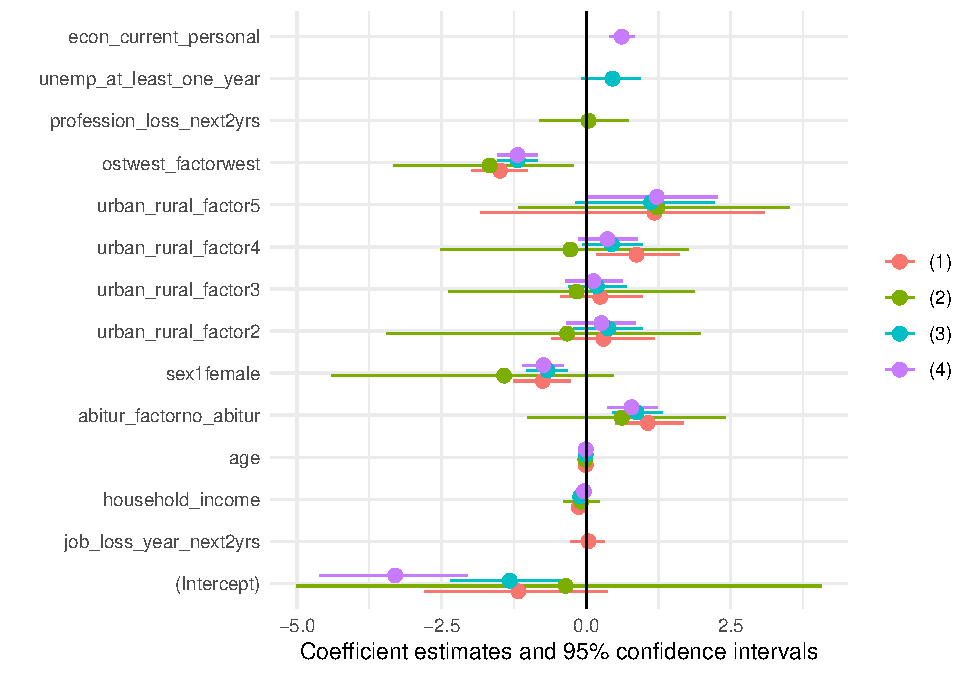
\includegraphics{AVCD_Final_Assignment-Edenhofer_latest_files/figure-latex/simple-models-insecurity-1.pdf}

\begin{Shaded}
\begin{Highlighting}[]
\CommentTok{\# simple models }
\DocumentationTok{\#\# difference gov}
\NormalTok{afd\_diff\_gov }\OtherTok{\textless{}{-}} \FunctionTok{glm}\NormalTok{(afd\_21 }\SpecialCharTok{\textasciitilde{}}\NormalTok{ difference\_whos\_gov }\SpecialCharTok{+}\NormalTok{ household\_income }\SpecialCharTok{+}\NormalTok{ age }\SpecialCharTok{+}\NormalTok{ abitur\_factor }\SpecialCharTok{+}\NormalTok{ sex1 }\SpecialCharTok{+}\NormalTok{ urban\_rural\_factor }\SpecialCharTok{+}\NormalTok{ ostwest\_factor, }\AttributeTok{family =} \FunctionTok{binomial}\NormalTok{(}\AttributeTok{link =} \StringTok{"logit"}\NormalTok{), }
                         \AttributeTok{data =}\NormalTok{ gles\_mod)}
\DocumentationTok{\#\# difference voting }
\NormalTok{afd\_prof\_loss\_fear }\OtherTok{\textless{}{-}} \FunctionTok{glm}\NormalTok{(afd\_21 }\SpecialCharTok{\textasciitilde{}}\NormalTok{ difference\_who\_votes }\SpecialCharTok{+}\NormalTok{ household\_income }\SpecialCharTok{+}\NormalTok{ age }\SpecialCharTok{+}\NormalTok{ abitur\_factor }\SpecialCharTok{+}\NormalTok{ sex1 }\SpecialCharTok{+}\NormalTok{ urban\_rural\_factor }\SpecialCharTok{+}\NormalTok{ ostwest\_factor, }\AttributeTok{family =} \FunctionTok{binomial}\NormalTok{(}\AttributeTok{link =} \StringTok{"logit"}\NormalTok{), }
                         \AttributeTok{data =}\NormalTok{ gles\_mod)}
\CommentTok{\# modelplot}
\FunctionTok{modelplot}\NormalTok{(}\FunctionTok{list}\NormalTok{(afd\_diff\_gov, afd\_prof\_loss\_fear)) }\SpecialCharTok{+}
  \FunctionTok{geom\_vline}\NormalTok{(}\AttributeTok{xintercept =} \DecValTok{0}\NormalTok{)}
\end{Highlighting}
\end{Shaded}

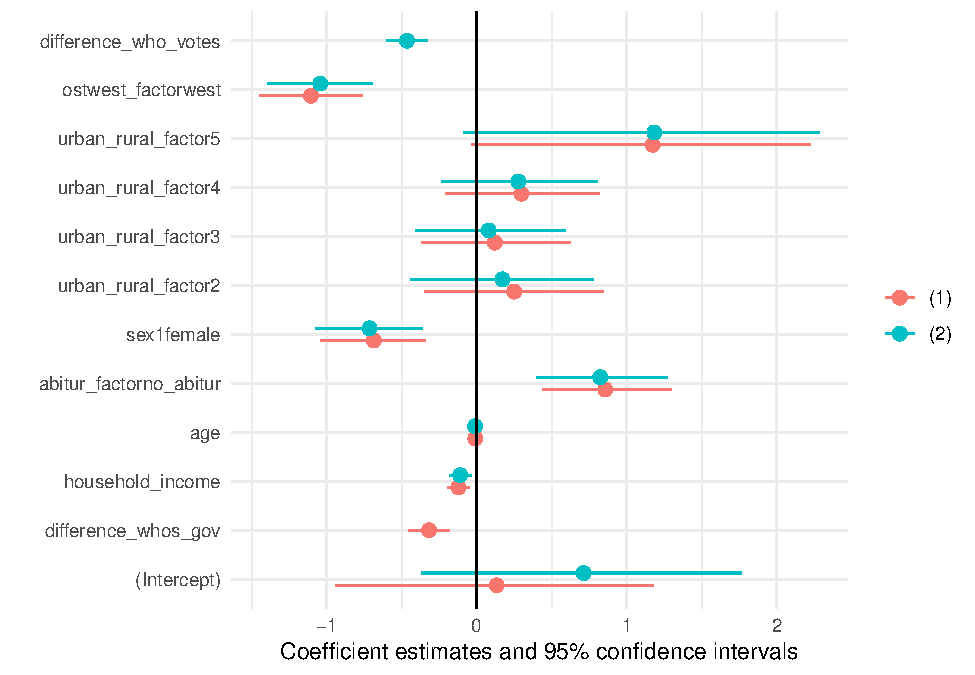
\includegraphics{AVCD_Final_Assignment-Edenhofer_latest_files/figure-latex/simple-models-lack-rep-1.pdf}

\begin{Shaded}
\begin{Highlighting}[]
\CommentTok{\# interaction models }
\DocumentationTok{\#\# difference gov}
\DocumentationTok{\#\#\# job loss fear }
\NormalTok{afd\_diff\_gov\_int1 }\OtherTok{\textless{}{-}} \FunctionTok{glm}\NormalTok{(afd\_21 }\SpecialCharTok{\textasciitilde{}}\NormalTok{ difference\_whos\_gov}\SpecialCharTok{*}\NormalTok{job\_loss\_year\_next2yrs }\SpecialCharTok{+}\NormalTok{ household\_income }\SpecialCharTok{+}\NormalTok{ age }\SpecialCharTok{+}\NormalTok{ abitur\_factor }\SpecialCharTok{+}\NormalTok{ sex1 }\SpecialCharTok{+}\NormalTok{ urban\_rural\_factor }\SpecialCharTok{+}\NormalTok{ ostwest\_factor, }\AttributeTok{family =} \FunctionTok{binomial}\NormalTok{(}\AttributeTok{link =} \StringTok{"logit"}\NormalTok{), }
                         \AttributeTok{data =}\NormalTok{ gles\_mod)}
\DocumentationTok{\#\#\# profession loss fear}
\NormalTok{afd\_diff\_gov\_int2 }\OtherTok{\textless{}{-}} \FunctionTok{glm}\NormalTok{(afd\_21 }\SpecialCharTok{\textasciitilde{}}\NormalTok{ difference\_whos\_gov}\SpecialCharTok{*}\NormalTok{profession\_loss\_next2yrs }\SpecialCharTok{+}\NormalTok{ household\_income }\SpecialCharTok{+}\NormalTok{ age }\SpecialCharTok{+}\NormalTok{ abitur\_factor }\SpecialCharTok{+}\NormalTok{ sex1 }\SpecialCharTok{+}\NormalTok{ urban\_rural\_factor }\SpecialCharTok{+}\NormalTok{ ostwest\_factor, }\AttributeTok{family =} \FunctionTok{binomial}\NormalTok{(}\AttributeTok{link =} \StringTok{"logit"}\NormalTok{), }
                         \AttributeTok{data =}\NormalTok{ gles\_mod)}
\DocumentationTok{\#\#\# unemployment experience}
\NormalTok{afd\_diff\_gov\_int3 }\OtherTok{\textless{}{-}} \FunctionTok{glm}\NormalTok{(afd\_21 }\SpecialCharTok{\textasciitilde{}}\NormalTok{ difference\_whos\_gov}\SpecialCharTok{*}\NormalTok{unemp\_at\_least\_one\_year }\SpecialCharTok{+}\NormalTok{ household\_income }\SpecialCharTok{+}\NormalTok{ age }\SpecialCharTok{+}\NormalTok{ abitur\_factor }\SpecialCharTok{+}\NormalTok{ sex1 }\SpecialCharTok{+}\NormalTok{ urban\_rural\_factor }\SpecialCharTok{+}\NormalTok{ ostwest\_factor, }\AttributeTok{family =} \FunctionTok{binomial}\NormalTok{(}\AttributeTok{link =} \StringTok{"logit"}\NormalTok{), }
                         \AttributeTok{data =}\NormalTok{ gles\_mod)}
\DocumentationTok{\#\#\# personal current situation}
\NormalTok{afd\_diff\_gov\_int4 }\OtherTok{\textless{}{-}} \FunctionTok{glm}\NormalTok{(afd\_21 }\SpecialCharTok{\textasciitilde{}}\NormalTok{ difference\_whos\_gov}\SpecialCharTok{*}\NormalTok{econ\_current\_personal }\SpecialCharTok{+}\NormalTok{ household\_income }\SpecialCharTok{+}\NormalTok{ age }\SpecialCharTok{+}\NormalTok{ abitur\_factor }\SpecialCharTok{+}\NormalTok{ sex1 }\SpecialCharTok{+}\NormalTok{ urban\_rural\_factor }\SpecialCharTok{+}\NormalTok{ ostwest\_factor, }\AttributeTok{family =} \FunctionTok{binomial}\NormalTok{(}\AttributeTok{link =} \StringTok{"logit"}\NormalTok{), }
                         \AttributeTok{data =}\NormalTok{ gles\_mod)}
\CommentTok{\# modelplot }
\FunctionTok{modelplot}\NormalTok{(}\FunctionTok{list}\NormalTok{(afd\_diff\_gov\_int1, afd\_diff\_gov\_int2, }
\NormalTok{               afd\_diff\_gov\_int3, afd\_diff\_gov\_int4)) }\SpecialCharTok{+}
  \FunctionTok{geom\_vline}\NormalTok{(}\AttributeTok{xintercept =} \DecValTok{0}\NormalTok{)}
\end{Highlighting}
\end{Shaded}

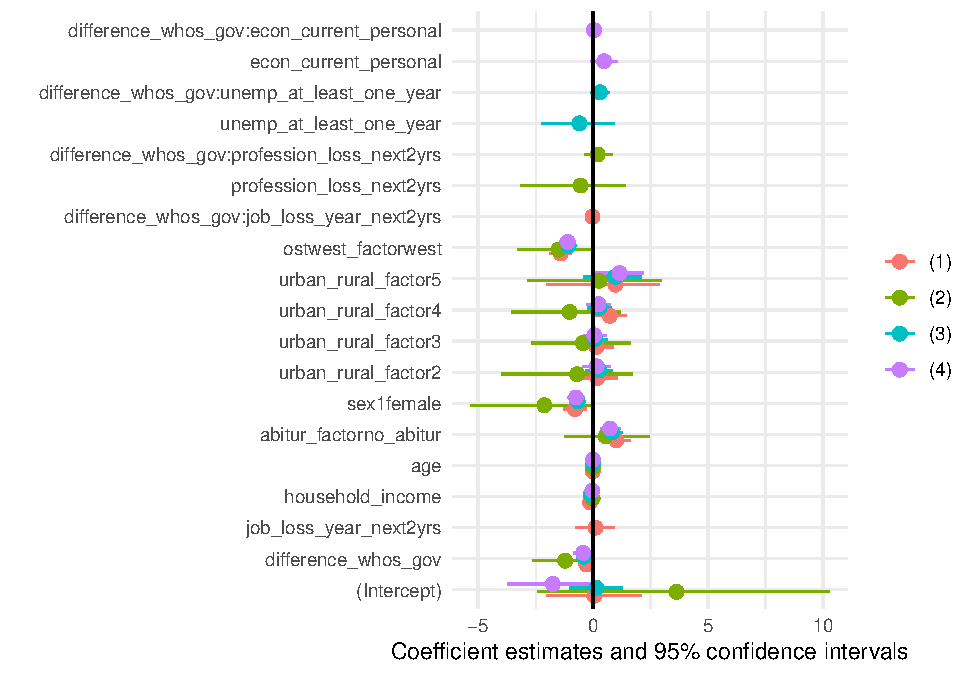
\includegraphics{AVCD_Final_Assignment-Edenhofer_latest_files/figure-latex/interaction-models-lack-rep-1.pdf}

\begin{Shaded}
\begin{Highlighting}[]
\CommentTok{\# models }
\DocumentationTok{\#\# trust in parliament}
\NormalTok{afd\_job\_loss\_fear\_int1 }\OtherTok{\textless{}{-}} \FunctionTok{glm}\NormalTok{(afd\_21 }\SpecialCharTok{\textasciitilde{}}\NormalTok{ job\_loss\_year\_next2yrs}\SpecialCharTok{*}\NormalTok{trust\_in\_parliament }\SpecialCharTok{+}\NormalTok{ household\_income }\SpecialCharTok{+}\NormalTok{ age }\SpecialCharTok{+}\NormalTok{ abitur\_factor }\SpecialCharTok{+}\NormalTok{ sex1 }\SpecialCharTok{+}\NormalTok{ urban\_rural\_factor }\SpecialCharTok{+}\NormalTok{ ostwest\_factor, }
                             \AttributeTok{family =} \FunctionTok{binomial}\NormalTok{(}\AttributeTok{link =} \StringTok{"logit"}\NormalTok{),}
                             \AttributeTok{data =}\NormalTok{ gles\_mod)}
\DocumentationTok{\#\# trust in parties }
\NormalTok{afd\_job\_loss\_fear\_int2 }\OtherTok{\textless{}{-}} \FunctionTok{glm}\NormalTok{(afd\_21 }\SpecialCharTok{\textasciitilde{}}\NormalTok{ job\_loss\_year\_next2yrs}\SpecialCharTok{*}\NormalTok{trust\_in\_parties }\SpecialCharTok{+}\NormalTok{ household\_income }\SpecialCharTok{+}\NormalTok{ age }\SpecialCharTok{+}\NormalTok{ abitur\_factor }\SpecialCharTok{+}\NormalTok{ sex1 }\SpecialCharTok{+}\NormalTok{ urban\_rural\_factor }\SpecialCharTok{+}\NormalTok{ ostwest\_factor, }
                             \AttributeTok{family =} \FunctionTok{binomial}\NormalTok{(}\AttributeTok{link =} \StringTok{"logit"}\NormalTok{),}
                             \AttributeTok{data =}\NormalTok{ gles\_mod)}
\DocumentationTok{\#\# trust in politicians}
\NormalTok{afd\_job\_loss\_fear\_int3 }\OtherTok{\textless{}{-}} \FunctionTok{glm}\NormalTok{(afd\_21 }\SpecialCharTok{\textasciitilde{}}\NormalTok{ job\_loss\_year\_next2yrs}\SpecialCharTok{*}\NormalTok{trust\_in\_politicians }\SpecialCharTok{+}\NormalTok{ household\_income }\SpecialCharTok{+}\NormalTok{ age }\SpecialCharTok{+}\NormalTok{ abitur\_factor }\SpecialCharTok{+}\NormalTok{ sex1 }\SpecialCharTok{+}\NormalTok{ urban\_rural\_factor }\SpecialCharTok{+}\NormalTok{ ostwest\_factor, }
                             \AttributeTok{family =} \FunctionTok{binomial}\NormalTok{(}\AttributeTok{link =} \StringTok{"logit"}\NormalTok{),}
                             \AttributeTok{data =}\NormalTok{ gles\_mod)}
\CommentTok{\# regression table }
\FunctionTok{modelsummary}\NormalTok{(}\FunctionTok{list}\NormalTok{(afd\_job\_loss\_fear\_int1, afd\_job\_loss\_fear\_int2, afd\_job\_loss\_fear\_int3),}
             \AttributeTok{estimate =} \StringTok{"\{estimate\}\{stars\}"}\NormalTok{)}
\end{Highlighting}
\end{Shaded}

\begin{table}
\centering
\begin{tabular}[t]{lccc}
\toprule
  & (1) & (2) & (3)\\
\midrule
(Intercept) & \num{0.376} & \num{0.765} & \num{0.153}\\
 & (\num{0.989}) & (\num{0.984}) & (\num{0.960})\\
job\_loss\_year\_next2yrs & \num{0.506} & \num{0.240} & \num{0.333}\\
 & (\num{0.343}) & (\num{0.349}) & (\num{0.337})\\
trust\_in\_parliament & \num{-0.160} &  & \\
 & (\num{0.169}) &  & \\
household\_income & \num{-0.080} & \num{-0.110}+ & \num{-0.112}+\\
 & (\num{0.067}) & (\num{0.065}) & (\num{0.064})\\
age & \num{-0.004} & \num{-0.006} & \num{-0.001}\\
 & (\num{0.011}) & (\num{0.011}) & (\num{0.011})\\
abitur\_factorno\_abitur & \num{0.959}** & \num{1.057}*** & \num{1.071}***\\
 & (\num{0.319}) & (\num{0.311}) & (\num{0.312})\\
sex1female & \num{-0.909}*** & \num{-0.937}*** & \num{-0.854}**\\
 & (\num{0.272}) & (\num{0.272}) & (\num{0.266})\\
urban\_rural\_factor2 & \num{-0.008} & \num{0.045} & \num{0.129}\\
 & (\num{0.485}) & (\num{0.479}) & (\num{0.477})\\
urban\_rural\_factor3 & \num{-0.225} & \num{0.076} & \num{0.067}\\
 & (\num{0.390}) & (\num{0.378}) & (\num{0.378})\\
urban\_rural\_factor4 & \num{0.584} & \num{0.646}+ & \num{0.659}+\\
 & (\num{0.381}) & (\num{0.373}) & (\num{0.374})\\
urban\_rural\_factor5 & \num{1.496} & \num{-13.252} & \num{1.370}\\
 & (\num{1.147}) & (\num{751.057}) & (\num{1.160})\\
ostwest\_factorwest & \num{-1.332}*** & \num{-1.308}*** & \num{-1.464}***\\
 & (\num{0.264}) & (\num{0.258}) & (\num{0.256})\\
job\_loss\_year\_next2yrs × trust\_in\_parliament & \num{-0.280}+ &  & \\
 & (\num{0.148}) &  & \\
trust\_in\_parties &  & \num{-0.404}** & \\
 &  & (\num{0.155}) & \\
job\_loss\_year\_next2yrs × trust\_in\_parties &  & \num{-0.119} & \\
 &  & (\num{0.114}) & \\
trust\_in\_politicians &  &  & \num{-0.320}*\\
 &  &  & (\num{0.152})\\
job\_loss\_year\_next2yrs × trust\_in\_politicians &  &  & \num{-0.148}\\
 &  &  & (\num{0.116})\\
\midrule
Num.Obs. & \num{1247} & \num{1242} & \num{1244}\\
AIC & \num{467.0} & \num{480.6} & \num{491.9}\\
BIC & \num{533.7} & \num{547.2} & \num{558.6}\\
Log.Lik. & \num{-220.509} & \num{-227.283} & \num{-232.956}\\
RMSE & \num{0.22} & \num{0.22} & \num{0.23}\\
\bottomrule
\end{tabular}
\end{table}

\begin{Shaded}
\begin{Highlighting}[]
\CommentTok{\# models }
\DocumentationTok{\#\# trust in parliament}
\NormalTok{afd\_prof\_loss\_fear\_int1 }\OtherTok{\textless{}{-}} \FunctionTok{glm}\NormalTok{(afd\_21 }\SpecialCharTok{\textasciitilde{}}\NormalTok{ profession\_loss\_next2yrs}\SpecialCharTok{*}\NormalTok{trust\_in\_parliament }\SpecialCharTok{+}\NormalTok{ household\_income }\SpecialCharTok{+}\NormalTok{ age }\SpecialCharTok{+}\NormalTok{ abitur\_factor }\SpecialCharTok{+}\NormalTok{ sex1 }\SpecialCharTok{+}\NormalTok{ urban\_rural\_factor }\SpecialCharTok{+}\NormalTok{ ostwest\_factor, }
                             \AttributeTok{family =} \FunctionTok{binomial}\NormalTok{(}\AttributeTok{link =} \StringTok{"logit"}\NormalTok{),}
                             \AttributeTok{data =}\NormalTok{ gles\_mod)}
\end{Highlighting}
\end{Shaded}

\begin{verbatim}
## Warning: glm.fit: fitted probabilities numerically 0 or 1 occurred
\end{verbatim}

\begin{Shaded}
\begin{Highlighting}[]
\DocumentationTok{\#\# trust in parties }
\NormalTok{afd\_prof\_loss\_fear\_int2 }\OtherTok{\textless{}{-}} \FunctionTok{glm}\NormalTok{(afd\_21 }\SpecialCharTok{\textasciitilde{}}\NormalTok{ profession\_loss\_next2yrs}\SpecialCharTok{*}\NormalTok{trust\_in\_parties }\SpecialCharTok{+}\NormalTok{ household\_income }\SpecialCharTok{+}\NormalTok{ age }\SpecialCharTok{+}\NormalTok{ abitur\_factor }\SpecialCharTok{+}\NormalTok{ sex1 }\SpecialCharTok{+}\NormalTok{ urban\_rural\_factor }\SpecialCharTok{+}\NormalTok{ ostwest\_factor, }
                             \AttributeTok{family =} \FunctionTok{binomial}\NormalTok{(}\AttributeTok{link =} \StringTok{"logit"}\NormalTok{),}
                             \AttributeTok{data =}\NormalTok{ gles\_mod)}
\end{Highlighting}
\end{Shaded}

\begin{verbatim}
## Warning: glm.fit: fitted probabilities numerically 0 or 1 occurred
\end{verbatim}

\begin{Shaded}
\begin{Highlighting}[]
\DocumentationTok{\#\# trust in politicians}
\NormalTok{afd\_prof\_loss\_fear\_int3 }\OtherTok{\textless{}{-}} \FunctionTok{glm}\NormalTok{(afd\_21 }\SpecialCharTok{\textasciitilde{}}\NormalTok{ profession\_loss\_next2yrs}\SpecialCharTok{*}\NormalTok{trust\_in\_politicians }\SpecialCharTok{+}\NormalTok{ household\_income }\SpecialCharTok{+}\NormalTok{ age }\SpecialCharTok{+}\NormalTok{ abitur\_factor }\SpecialCharTok{+}\NormalTok{ sex1 }\SpecialCharTok{+}\NormalTok{ urban\_rural\_factor }\SpecialCharTok{+}\NormalTok{ ostwest\_factor, }
                             \AttributeTok{family =} \FunctionTok{binomial}\NormalTok{(}\AttributeTok{link =} \StringTok{"logit"}\NormalTok{),}
                             \AttributeTok{data =}\NormalTok{ gles\_mod)}
\end{Highlighting}
\end{Shaded}

\begin{verbatim}
## Warning: glm.fit: fitted probabilities numerically 0 or 1 occurred
\end{verbatim}

\begin{Shaded}
\begin{Highlighting}[]
\CommentTok{\# regression table }
\FunctionTok{modelsummary}\NormalTok{(}\FunctionTok{list}\NormalTok{(afd\_prof\_loss\_fear\_int1, afd\_prof\_loss\_fear\_int2, afd\_prof\_loss\_fear\_int3),}
             \AttributeTok{estimate =} \StringTok{"\{estimate\}\{stars\}"}\NormalTok{)}
\end{Highlighting}
\end{Shaded}

\begin{table}
\centering
\begin{tabular}[t]{lccc}
\toprule
  & (1) & (2) & (3)\\
\midrule
(Intercept) & \num{-49.880} & \num{-1.123} & \num{-7.002}\\
 & (\num{5687.044}) & (\num{3.719}) & (\num{974.853})\\
profession\_loss\_next2yrs & \num{44.364} & \num{2.110} & \num{7.241}\\
 & (\num{5687.037}) & (\num{1.659}) & (\num{974.848})\\
trust\_in\_parliament & \num{20.849} &  & \\
 & (\num{2843.518}) &  \vphantom{1} & \\
household\_income & \num{0.768} & \num{0.136} & \num{0.173}\\
 & (\num{0.493}) & (\num{0.227}) & (\num{0.233})\\
age & \num{-0.039} & \num{-0.046} & \num{-0.033}\\
 & (\num{0.057}) & (\num{0.049}) & (\num{0.048})\\
abitur\_factorno\_abitur & \num{1.344} & \num{1.013} & \num{0.889}\\
 & (\num{1.143}) & (\num{1.048}) & (\num{1.026})\\
sex1female & \num{-21.845} & \num{-17.891} & \num{-20.004}\\
 & (\num{13548.639}) & (\num{1978.524}) & (\num{5283.111})\\
urban\_rural\_factor2 & \num{0.044} & \num{-0.357} & \num{-0.457}\\
 & (\num{1.593}) & (\num{1.446}) & (\num{1.506})\\
urban\_rural\_factor3 & \num{1.567} & \num{0.563} & \num{0.796}\\
 & (\num{1.450}) & (\num{1.181}) & (\num{1.214})\\
urban\_rural\_factor4 & \num{-0.530} & \num{-1.627} & \num{-1.656}\\
 & (\num{1.530}) & (\num{1.512}) & (\num{1.530})\\
urban\_rural\_factor5 & \num{3.433} & \num{2.063} & \num{1.934}\\
 & (\num{2.259}) & (\num{1.528}) & (\num{1.656})\\
ostwest\_factorwest & \num{-1.564} & \num{-1.439} & \num{-1.267}\\
 & (\num{1.074}) & (\num{0.929}) & (\num{0.949})\\
profession\_loss\_next2yrs × trust\_in\_parliament & \num{-21.450} &  & \\
 & (\num{2843.518}) &  & \\
trust\_in\_parties &  & \num{0.371} & \\
 &  & (\num{0.763}) & \\
profession\_loss\_next2yrs × trust\_in\_parties &  & \num{-0.825} & \\
 &  & (\num{0.673}) & \\
trust\_in\_politicians &  &  & \num{5.726}\\
 &  &  & \vphantom{1} (\num{974.847})\\
profession\_loss\_next2yrs × trust\_in\_politicians &  &  & \num{-6.253}\\
 &  &  & (\num{974.847})\\
\midrule
Num.Obs. & \num{155} & \num{156} & \num{155}\\
AIC & \num{58.5} & \num{66.2} & \num{63.1}\\
BIC & \num{98.0} & \num{105.9} & \num{102.7}\\
Log.Lik. & \num{-16.227} & \num{-20.123} & \num{-18.554}\\
RMSE & \num{0.18} & \num{0.18} & \num{0.18}\\
\bottomrule
\end{tabular}
\end{table}

\begin{Shaded}
\begin{Highlighting}[]
\CommentTok{\# models }
\DocumentationTok{\#\# trust in parliament}
\NormalTok{afd\_unemp\_exp\_int1 }\OtherTok{\textless{}{-}} \FunctionTok{glm}\NormalTok{(afd\_21 }\SpecialCharTok{\textasciitilde{}}\NormalTok{ unemp\_at\_least\_one\_year}\SpecialCharTok{*}\NormalTok{trust\_in\_parliament }\SpecialCharTok{+}\NormalTok{ household\_income }\SpecialCharTok{+}\NormalTok{ age }\SpecialCharTok{+}\NormalTok{ abitur\_factor }\SpecialCharTok{+}\NormalTok{ sex1 }\SpecialCharTok{+}\NormalTok{ urban\_rural\_factor }\SpecialCharTok{+}\NormalTok{ ostwest\_factor, }
                             \AttributeTok{family =} \FunctionTok{binomial}\NormalTok{(}\AttributeTok{link =} \StringTok{"logit"}\NormalTok{),}
                             \AttributeTok{data =}\NormalTok{ gles\_mod)}
\DocumentationTok{\#\# trust in parties }
\NormalTok{afd\_unemp\_exp\_int2 }\OtherTok{\textless{}{-}} \FunctionTok{glm}\NormalTok{(afd\_21 }\SpecialCharTok{\textasciitilde{}}\NormalTok{ unemp\_at\_least\_one\_year}\SpecialCharTok{*}\NormalTok{trust\_in\_parties }\SpecialCharTok{+}\NormalTok{ household\_income }\SpecialCharTok{+}\NormalTok{ age }\SpecialCharTok{+}\NormalTok{ abitur\_factor }\SpecialCharTok{+}\NormalTok{ sex1 }\SpecialCharTok{+}\NormalTok{ urban\_rural\_factor }\SpecialCharTok{+}\NormalTok{ ostwest\_factor, }
                             \AttributeTok{family =} \FunctionTok{binomial}\NormalTok{(}\AttributeTok{link =} \StringTok{"logit"}\NormalTok{),}
                             \AttributeTok{data =}\NormalTok{ gles\_mod)}
\DocumentationTok{\#\# trust in politicians}
\NormalTok{afd\_unemp\_exp\_int3 }\OtherTok{\textless{}{-}} \FunctionTok{glm}\NormalTok{(afd\_21 }\SpecialCharTok{\textasciitilde{}}\NormalTok{ unemp\_at\_least\_one\_year}\SpecialCharTok{*}\NormalTok{trust\_in\_politicians }\SpecialCharTok{+}\NormalTok{ household\_income }\SpecialCharTok{+}\NormalTok{ age }\SpecialCharTok{+}\NormalTok{ abitur\_factor }\SpecialCharTok{+}\NormalTok{ sex1 }\SpecialCharTok{+}\NormalTok{ urban\_rural\_factor }\SpecialCharTok{+}\NormalTok{ ostwest\_factor, }
                             \AttributeTok{family =} \FunctionTok{binomial}\NormalTok{(}\AttributeTok{link =} \StringTok{"logit"}\NormalTok{),}
                             \AttributeTok{data =}\NormalTok{ gles\_mod)}
\CommentTok{\# regression table }
\FunctionTok{modelsummary}\NormalTok{(}\FunctionTok{list}\NormalTok{(afd\_unemp\_exp\_int1, afd\_unemp\_exp\_int2, afd\_unemp\_exp\_int3),}
             \AttributeTok{estimate =} \StringTok{"\{estimate\}\{stars\}"}\NormalTok{)}
\end{Highlighting}
\end{Shaded}

\begin{table}
\centering
\begin{tabular}[t]{lccc}
\toprule
  & (1) & (2) & (3)\\
\midrule
(Intercept) & \num{0.428} & \num{0.906} & \num{0.434}\\
 & (\num{0.618}) & (\num{0.606}) & (\num{0.599})\\
unemp\_at\_least\_one\_year & \num{1.066}+ & \num{0.360} & \num{0.537}\\
 & (\num{0.600}) & (\num{0.621}) & (\num{0.579})\\
trust\_in\_parliament & \num{-0.493}*** &  & \\
 & (\num{0.045}) &  & \\
household\_income & \num{-0.049} & \num{-0.082}+ & \num{-0.074}+\\
 & (\num{0.044}) & (\num{0.042}) & (\num{0.043})\\
age & \num{0.003} & \num{-0.004} & \num{0.000}\\
 & (\num{0.006}) & (\num{0.006}) & (\num{0.006})\\
abitur\_factorno\_abitur & \num{0.670}** & \num{0.802}*** & \num{0.779}***\\
 & (\num{0.234}) & (\num{0.231}) & (\num{0.231})\\
sex1female & \num{-0.822}*** & \num{-0.825}*** & \num{-0.763}***\\
 & (\num{0.202}) & (\num{0.199}) & (\num{0.197})\\
urban\_rural\_factor2 & \num{0.098} & \num{0.105} & \num{0.130}\\
 & (\num{0.331}) & (\num{0.325}) & (\num{0.325})\\
urban\_rural\_factor3 & \num{-0.046} & \num{0.039} & \num{0.015}\\
 & (\num{0.278}) & (\num{0.272}) & (\num{0.272})\\
urban\_rural\_factor4 & \num{0.287} & \num{0.270} & \num{0.268}\\
 & (\num{0.285}) & (\num{0.279}) & (\num{0.279})\\
urban\_rural\_factor5 & \num{1.241}+ & \num{0.685} & \num{1.226}+\\
 & (\num{0.691}) & (\num{0.709}) & (\num{0.661})\\
ostwest\_factorwest & \num{-1.075}*** & \num{-1.073}*** & \num{-1.148}***\\
 & (\num{0.193}) & (\num{0.190}) & (\num{0.189})\\
unemp\_at\_least\_one\_year × trust\_in\_parliament & \num{-0.211} &  & \\
 & (\num{0.153}) &  & \\
trust\_in\_parties &  & \num{-0.577}*** & \\
 &  & (\num{0.059}) & \\
unemp\_at\_least\_one\_year × trust\_in\_parties &  & \num{0.000} & \\
 &  & (\num{0.163}) & \\
trust\_in\_politicians &  &  & \num{-0.539}***\\
 &  &  & (\num{0.056})\\
unemp\_at\_least\_one\_year × trust\_in\_politicians &  &  & \num{-0.076}\\
 &  &  & (\num{0.165})\\
\midrule
Num.Obs. & \num{2272} & \num{2263} & \num{2266}\\
AIC & \num{840.2} & \num{870.5} & \num{875.9}\\
BIC & \num{914.7} & \num{944.9} & \num{950.3}\\
Log.Lik. & \num{-407.109} & \num{-422.250} & \num{-424.940}\\
RMSE & \num{0.22} & \num{0.23} & \num{0.23}\\
\bottomrule
\end{tabular}
\end{table}

\begin{Shaded}
\begin{Highlighting}[]
\CommentTok{\# models }
\DocumentationTok{\#\# trust in parliament}
\NormalTok{afd\_econ\_current\_int1 }\OtherTok{\textless{}{-}} \FunctionTok{glm}\NormalTok{(afd\_21 }\SpecialCharTok{\textasciitilde{}}\NormalTok{ econ\_current\_personal}\SpecialCharTok{*}\NormalTok{trust\_in\_parliament }\SpecialCharTok{+}\NormalTok{ household\_income }\SpecialCharTok{+}\NormalTok{ age }\SpecialCharTok{+}\NormalTok{ abitur\_factor }\SpecialCharTok{+}\NormalTok{ sex1 }\SpecialCharTok{+}\NormalTok{ urban\_rural\_factor }\SpecialCharTok{+}\NormalTok{ ostwest\_factor, }
                             \AttributeTok{family =} \FunctionTok{binomial}\NormalTok{(}\AttributeTok{link =} \StringTok{"logit"}\NormalTok{),}
                             \AttributeTok{data =}\NormalTok{ gles\_mod)}
\DocumentationTok{\#\# trust in parties }
\NormalTok{afd\_econ\_current\_int2 }\OtherTok{\textless{}{-}} \FunctionTok{glm}\NormalTok{(afd\_21 }\SpecialCharTok{\textasciitilde{}}\NormalTok{ econ\_current\_personal}\SpecialCharTok{*}\NormalTok{trust\_in\_parties }\SpecialCharTok{+}\NormalTok{ household\_income }\SpecialCharTok{+}\NormalTok{ age }\SpecialCharTok{+}\NormalTok{ abitur\_factor }\SpecialCharTok{+}\NormalTok{ sex1 }\SpecialCharTok{+}\NormalTok{ urban\_rural\_factor }\SpecialCharTok{+}\NormalTok{ ostwest\_factor, }
                             \AttributeTok{family =} \FunctionTok{binomial}\NormalTok{(}\AttributeTok{link =} \StringTok{"logit"}\NormalTok{),}
                             \AttributeTok{data =}\NormalTok{ gles\_mod)}
\DocumentationTok{\#\# trust in politicians}
\NormalTok{afd\_econ\_current\_int3 }\OtherTok{\textless{}{-}} \FunctionTok{glm}\NormalTok{(afd\_21 }\SpecialCharTok{\textasciitilde{}}\NormalTok{ econ\_current\_personal}\SpecialCharTok{*}\NormalTok{trust\_in\_politicians }\SpecialCharTok{+}\NormalTok{ household\_income }\SpecialCharTok{+}\NormalTok{ age }\SpecialCharTok{+}\NormalTok{ abitur\_factor }\SpecialCharTok{+}\NormalTok{ sex1 }\SpecialCharTok{+}\NormalTok{ urban\_rural\_factor }\SpecialCharTok{+}\NormalTok{ ostwest\_factor, }
                             \AttributeTok{family =} \FunctionTok{binomial}\NormalTok{(}\AttributeTok{link =} \StringTok{"logit"}\NormalTok{),}
                             \AttributeTok{data =}\NormalTok{ gles\_mod)}
\CommentTok{\# regression table }
\FunctionTok{modelsummary}\NormalTok{(}\FunctionTok{list}\NormalTok{(afd\_econ\_current\_int1, afd\_econ\_current\_int2, afd\_econ\_current\_int3),}
             \AttributeTok{estimate =} \StringTok{"\{estimate\}\{stars\}"}\NormalTok{)}
\end{Highlighting}
\end{Shaded}

\begin{table}
\centering
\begin{tabular}[t]{lccc}
\toprule
  & (1) & (2) & (3)\\
\midrule
(Intercept) & \num{-1.341} & \num{-1.939}* & \num{-2.230}*\\
 & (\num{0.923}) & (\num{0.953}) & (\num{0.915})\\
econ\_current\_personal & \num{0.611}** & \num{0.892}*** & \num{0.844}***\\
 & (\num{0.210}) & (\num{0.236}) & (\num{0.216})\\
trust\_in\_parliament & \num{-0.242}* &  & \\
 & (\num{0.120}) &  & \\
household\_income & \num{-0.022} & \num{-0.025} & \num{-0.018}\\
 & (\num{0.046}) & (\num{0.045}) & (\num{0.045})\\
age & \num{0.003} & \num{-0.002} & \num{0.001}\\
 & (\num{0.006}) & (\num{0.006}) & (\num{0.006})\\
abitur\_factorno\_abitur & \num{0.691}** & \num{0.796}*** & \num{0.812}***\\
 & (\num{0.234}) & (\num{0.231}) & (\num{0.231})\\
sex1female & \num{-0.883}*** & \num{-0.940}*** & \num{-0.891}***\\
 & (\num{0.201}) & (\num{0.202}) & (\num{0.200})\\
urban\_rural\_factor2 & \num{0.059} & \num{0.092} & \num{0.107}\\
 & (\num{0.328}) & (\num{0.326}) & (\num{0.324})\\
urban\_rural\_factor3 & \num{-0.006} & \num{0.080} & \num{0.032}\\
 & (\num{0.276}) & (\num{0.273}) & (\num{0.272})\\
urban\_rural\_factor4 & \num{0.299} & \num{0.247} & \num{0.259}\\
 & (\num{0.282}) & (\num{0.280}) & (\num{0.279})\\
urban\_rural\_factor5 & \num{1.500}* & \num{0.876} & \num{1.368}*\\
 & (\num{0.627}) & (\num{0.649}) & (\num{0.618})\\
ostwest\_factorwest & \num{-1.090}*** & \num{-1.130}*** & \num{-1.187}***\\
 & (\num{0.191}) & (\num{0.189}) & (\num{0.188})\\
econ\_current\_personal × trust\_in\_parliament & \num{-0.103}* &  & \\
 & (\num{0.047}) &  & \\
trust\_in\_parties &  & \num{-0.177} & \\
 &  & (\num{0.156}) & \\
econ\_current\_personal × trust\_in\_parties &  & \num{-0.146}* & \\
 &  & (\num{0.060}) & \\
trust\_in\_politicians &  &  & \num{-0.176}\\
 &  &  & (\num{0.147})\\
econ\_current\_personal × trust\_in\_politicians &  &  & \num{-0.140}*\\
 &  &  & (\num{0.058})\\
\midrule
Num.Obs. & \num{2351} & \num{2341} & \num{2346}\\
AIC & \num{866.9} & \num{890.4} & \num{894.3}\\
BIC & \num{941.8} & \num{965.3} & \num{969.2}\\
Log.Lik. & \num{-420.467} & \num{-432.214} & \num{-434.139}\\
F &  & \num{16.825} & \num{16.786}\\
RMSE & \num{0.22} & \num{0.22} & \num{0.23}\\
\bottomrule
\end{tabular}
\end{table}

\hypertarget{conclusion}{%
\section{Conclusion}\label{conclusion}}

\hypertarget{references}{%
\section{References}\label{references}}

\hypertarget{appendix}{%
\section{Appendix}\label{appendix}}

\hypertarget{analysis---afd}{%
\section{Analysis - AfD}\label{analysis---afd}}

\hypertarget{socio-demographic-correlates}{%
\subsubsection{Socio-demographic
Correlates}\label{socio-demographic-correlates}}

Relationship between household income and AfD voting

\begin{Shaded}
\begin{Highlighting}[]
\NormalTok{afd\_income }\OtherTok{\textless{}{-}} \FunctionTok{glm}\NormalTok{(afd\_21 }\SpecialCharTok{\textasciitilde{}}\NormalTok{ household\_income }\SpecialCharTok{+}\NormalTok{ age }\SpecialCharTok{+}\NormalTok{ abitur\_factor }\SpecialCharTok{+}\NormalTok{ sex1 }\SpecialCharTok{+}\NormalTok{ urban\_rural\_factor }\SpecialCharTok{+}\NormalTok{ ostwest\_factor, }\AttributeTok{family =} \FunctionTok{binomial}\NormalTok{(}\AttributeTok{link =} \StringTok{"logit"}\NormalTok{), }\AttributeTok{data =}\NormalTok{ gles\_mod)}
\FunctionTok{cplot}\NormalTok{(afd\_income, }\AttributeTok{x =} \StringTok{"household\_income"}\NormalTok{,}
      \AttributeTok{xvals =} \FunctionTok{seq}\NormalTok{(}\DecValTok{1}\NormalTok{, }\DecValTok{13}\NormalTok{, }\DecValTok{1}\NormalTok{), }\AttributeTok{draw =}\NormalTok{ F) }\SpecialCharTok{\%\textgreater{}\%}
  \FunctionTok{as\_tibble}\NormalTok{() }\SpecialCharTok{\%\textgreater{}\%}
  \FunctionTok{ggplot}\NormalTok{(}\FunctionTok{aes}\NormalTok{(}\AttributeTok{x =}\NormalTok{ xvals)) }\SpecialCharTok{+}
  \FunctionTok{geom\_point}\NormalTok{(}\FunctionTok{aes}\NormalTok{(}\AttributeTok{y =}\NormalTok{ yvals)) }\SpecialCharTok{+}
  \FunctionTok{geom\_errorbar}\NormalTok{(}\FunctionTok{aes}\NormalTok{(}\AttributeTok{ymin =}\NormalTok{ lower, }\AttributeTok{ymax =}\NormalTok{ upper), }\AttributeTok{width =} \FloatTok{0.2}\NormalTok{) }\SpecialCharTok{+}
  \FunctionTok{scale\_x\_continuous}\NormalTok{(}\StringTok{"Net Monthly Household Income"}\NormalTok{,}
                     \AttributeTok{breaks =} \FunctionTok{seq}\NormalTok{(}\DecValTok{1}\NormalTok{, }\DecValTok{13}\NormalTok{, }\DecValTok{1}\NormalTok{),}
                     \AttributeTok{labels =} \FunctionTok{c}\NormalTok{(}\StringTok{"\textless{}500€"}\NormalTok{, }\StringTok{"[500{-}750€)"}\NormalTok{,}
                                \StringTok{"[750{-}1000€)"}\NormalTok{, }\StringTok{"[1000{-}1250€)"}\NormalTok{, }
                                \StringTok{"[1250{-}1500€)"}\NormalTok{, }\StringTok{"[1500{-}2000€)"}\NormalTok{,}
                                \StringTok{"[2000{-}2500€)"}\NormalTok{, }\StringTok{"[2500{-}3000€)"}\NormalTok{,}
                                \StringTok{"[3000{-}4000€)"}\NormalTok{, }\StringTok{"[4000{-}5000€)"}\NormalTok{,}
                                \StringTok{"[5000{-}7000€)"}\NormalTok{, }\StringTok{"[7000{-}10000€)"}\NormalTok{,}
                                \StringTok{"\textgreater{}10000€"}\NormalTok{)) }\SpecialCharTok{+}
  \FunctionTok{labs}\NormalTok{(}\AttributeTok{y =} \StringTok{"Predicted Probability of Voting for the AfD"}\NormalTok{) }\SpecialCharTok{+}
  \FunctionTok{ylim}\NormalTok{(}\FunctionTok{c}\NormalTok{(}\DecValTok{0}\NormalTok{, }\FloatTok{0.3}\NormalTok{)) }\SpecialCharTok{+}
  \FunctionTok{theme\_bw}\NormalTok{() }\SpecialCharTok{+}
  \FunctionTok{theme}\NormalTok{(}\AttributeTok{axis.text.x =} \FunctionTok{element\_text}\NormalTok{(}\AttributeTok{angle =} \DecValTok{15}\NormalTok{, }\AttributeTok{hjust =} \DecValTok{1}\NormalTok{))}
\end{Highlighting}
\end{Shaded}

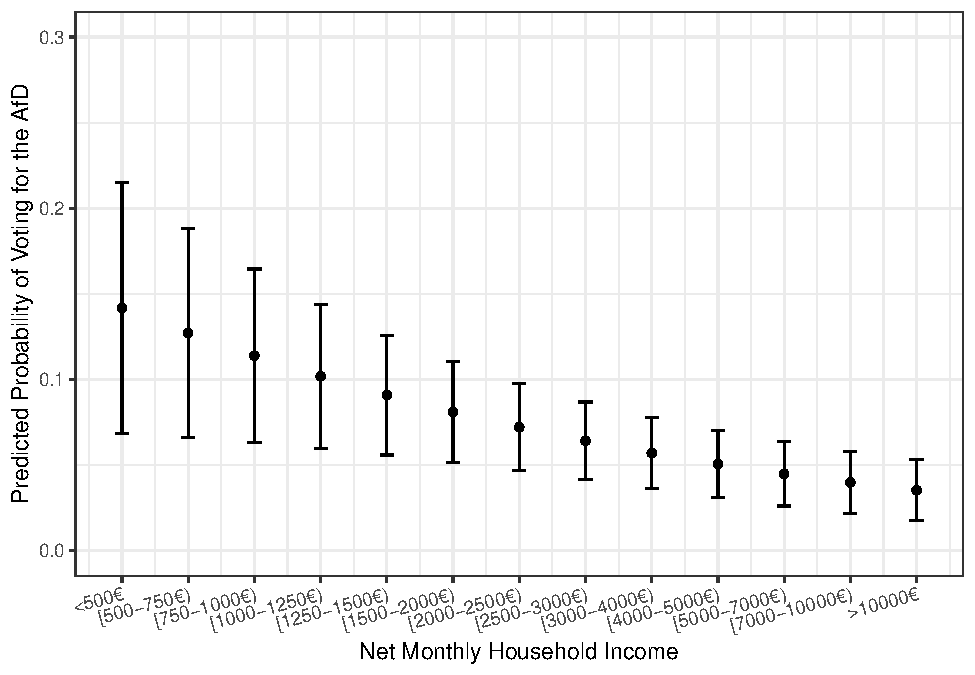
\includegraphics{AVCD_Final_Assignment-Edenhofer_latest_files/figure-latex/afd-household-income-1.pdf}

Relationship between subjective class and AfD voting

\begin{Shaded}
\begin{Highlighting}[]
\CommentTok{\# model}
\NormalTok{afd\_class }\OtherTok{\textless{}{-}} \FunctionTok{glm}\NormalTok{(afd\_21 }\SpecialCharTok{\textasciitilde{}}\NormalTok{ subjective\_class }\SpecialCharTok{+}\NormalTok{ age }\SpecialCharTok{+}\NormalTok{ abitur\_factor }\SpecialCharTok{+}\NormalTok{ sex1 }\SpecialCharTok{+}\NormalTok{ urban\_rural\_factor }\SpecialCharTok{+}\NormalTok{ ostwest\_factor, }\AttributeTok{family =} \FunctionTok{binomial}\NormalTok{(}\AttributeTok{link =} \StringTok{"logit"}\NormalTok{), }\AttributeTok{data =}\NormalTok{ gles\_mod)}
\CommentTok{\# plot}
\FunctionTok{cplot}\NormalTok{(afd\_class, }\AttributeTok{x =} \StringTok{"subjective\_class"}\NormalTok{, }
      \AttributeTok{xvals =} \FunctionTok{seq}\NormalTok{(}\DecValTok{1}\NormalTok{, }\DecValTok{6}\NormalTok{, }\DecValTok{1}\NormalTok{), }\AttributeTok{draw =}\NormalTok{ F) }\SpecialCharTok{\%\textgreater{}\%}
  \FunctionTok{as\_tibble}\NormalTok{() }\SpecialCharTok{\%\textgreater{}\%}
  \FunctionTok{ggplot}\NormalTok{(}\FunctionTok{aes}\NormalTok{(}\AttributeTok{x =}\NormalTok{ xvals)) }\SpecialCharTok{+}
  \FunctionTok{geom\_point}\NormalTok{(}\FunctionTok{aes}\NormalTok{(}\AttributeTok{y =}\NormalTok{ yvals)) }\SpecialCharTok{+}
  \FunctionTok{geom\_errorbar}\NormalTok{(}\FunctionTok{aes}\NormalTok{(}\AttributeTok{ymin =}\NormalTok{ lower, }\AttributeTok{ymax =}\NormalTok{ upper), }\AttributeTok{width =} \FloatTok{0.2}\NormalTok{) }\SpecialCharTok{+}
  \FunctionTok{scale\_x\_continuous}\NormalTok{(}\StringTok{"Subjective Class"}\NormalTok{, }
                     \AttributeTok{breaks =} \FunctionTok{seq}\NormalTok{(}\DecValTok{1}\NormalTok{, }\DecValTok{6}\NormalTok{, }\DecValTok{1}\NormalTok{), }
                     \AttributeTok{labels =} \FunctionTok{c}\NormalTok{(}\StringTok{"Unterschicht"}\NormalTok{, }\StringTok{"Arbeiterschicht"}\NormalTok{, }
                                \StringTok{"Untere Mittelschicht"}\NormalTok{, }\StringTok{"mittlere Mittelschicht"}\NormalTok{, }\StringTok{"obere Mittelschicht"}\NormalTok{, }\StringTok{"Oberschicht"}\NormalTok{)) }\SpecialCharTok{+}
  \FunctionTok{labs}\NormalTok{(}\AttributeTok{y =} \StringTok{"Predicted Probability of Voting AfD"}\NormalTok{) }\SpecialCharTok{+}
  \FunctionTok{expand\_limits}\NormalTok{(}\AttributeTok{y =} \FloatTok{0.4}\NormalTok{) }\SpecialCharTok{+}
  \FunctionTok{theme\_bw}\NormalTok{() }\SpecialCharTok{+}
  \FunctionTok{theme}\NormalTok{(}\AttributeTok{axis.text.x =} \FunctionTok{element\_text}\NormalTok{(}\AttributeTok{angle =} \DecValTok{15}\NormalTok{, }\AttributeTok{hjust =} \DecValTok{1}\NormalTok{))}
\end{Highlighting}
\end{Shaded}

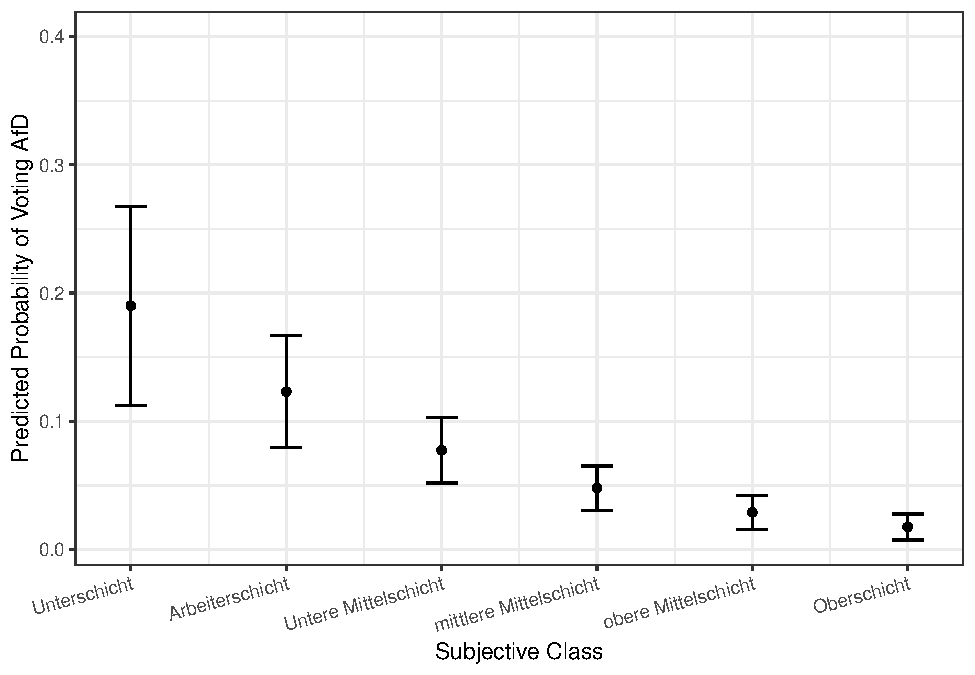
\includegraphics{AVCD_Final_Assignment-Edenhofer_latest_files/figure-latex/afd-subjective-class-1.pdf}

What is the relationship between left-right self-placement and AfD
voting?

\begin{Shaded}
\begin{Highlighting}[]
\NormalTok{afd\_left\_right\_placement }\OtherTok{\textless{}{-}} \FunctionTok{glm}\NormalTok{(afd\_21 }\SpecialCharTok{\textasciitilde{}}\NormalTok{ left\_right\_self }\SpecialCharTok{+} \FunctionTok{I}\NormalTok{(left\_right\_self}\SpecialCharTok{\^{}}\DecValTok{2}\NormalTok{) }\SpecialCharTok{+}\NormalTok{ household\_income }\SpecialCharTok{+}\NormalTok{ age }\SpecialCharTok{+}\NormalTok{ abitur\_factor }\SpecialCharTok{+}\NormalTok{ sex1 }\SpecialCharTok{+}\NormalTok{ urban\_rural\_factor }\SpecialCharTok{+}\NormalTok{ ostwest\_factor, }\AttributeTok{family =} \FunctionTok{binomial}\NormalTok{(}\AttributeTok{link =} \StringTok{"logit"}\NormalTok{), }\AttributeTok{data =}\NormalTok{ gles\_mod)}
\CommentTok{\# plot this model }
\FunctionTok{cplot}\NormalTok{(afd\_left\_right\_placement, }\AttributeTok{x =} \StringTok{"left\_right\_self"}\NormalTok{, }
      \AttributeTok{xvals =} \FunctionTok{seq}\NormalTok{(}\DecValTok{1}\NormalTok{, }\DecValTok{11}\NormalTok{, }\DecValTok{1}\NormalTok{), }\AttributeTok{draw =}\NormalTok{ F) }\SpecialCharTok{\%\textgreater{}\%}
  \FunctionTok{as\_tibble}\NormalTok{() }\SpecialCharTok{\%\textgreater{}\%}
  \FunctionTok{ggplot}\NormalTok{(}\FunctionTok{aes}\NormalTok{(}\AttributeTok{x =}\NormalTok{ xvals)) }\SpecialCharTok{+}
  \FunctionTok{geom\_point}\NormalTok{(}\FunctionTok{aes}\NormalTok{(}\AttributeTok{y =}\NormalTok{ yvals)) }\SpecialCharTok{+}
  \FunctionTok{geom\_errorbar}\NormalTok{(}\FunctionTok{aes}\NormalTok{(}\AttributeTok{ymin =}\NormalTok{ lower, }\AttributeTok{ymax =}\NormalTok{ upper), }\AttributeTok{width =} \FloatTok{0.2}\NormalTok{) }\SpecialCharTok{+}
  \FunctionTok{scale\_x\_continuous}\NormalTok{(}\StringTok{"Left{-}Right Self{-}Placement"}\NormalTok{, }
                     \AttributeTok{breaks =} \FunctionTok{seq}\NormalTok{(}\DecValTok{1}\NormalTok{, }\DecValTok{11}\NormalTok{, }\DecValTok{1}\NormalTok{)) }\SpecialCharTok{+}
  \FunctionTok{expand\_limits}\NormalTok{(}\AttributeTok{y =} \FloatTok{0.3}\NormalTok{) }\SpecialCharTok{+}
  \FunctionTok{labs}\NormalTok{(}\AttributeTok{y =} \StringTok{"Predicted Probability of Voting AfD"}\NormalTok{, }
       \AttributeTok{caption =} \StringTok{"\textquotesingle{}1\textquotesingle{} indicates respondents who locate themselves on the left of the ideological spectrum, while \textquotesingle{}11\textquotesingle{} indicates the opposite."}\NormalTok{) }\SpecialCharTok{+}
  \FunctionTok{theme\_bw}\NormalTok{()}
\end{Highlighting}
\end{Shaded}

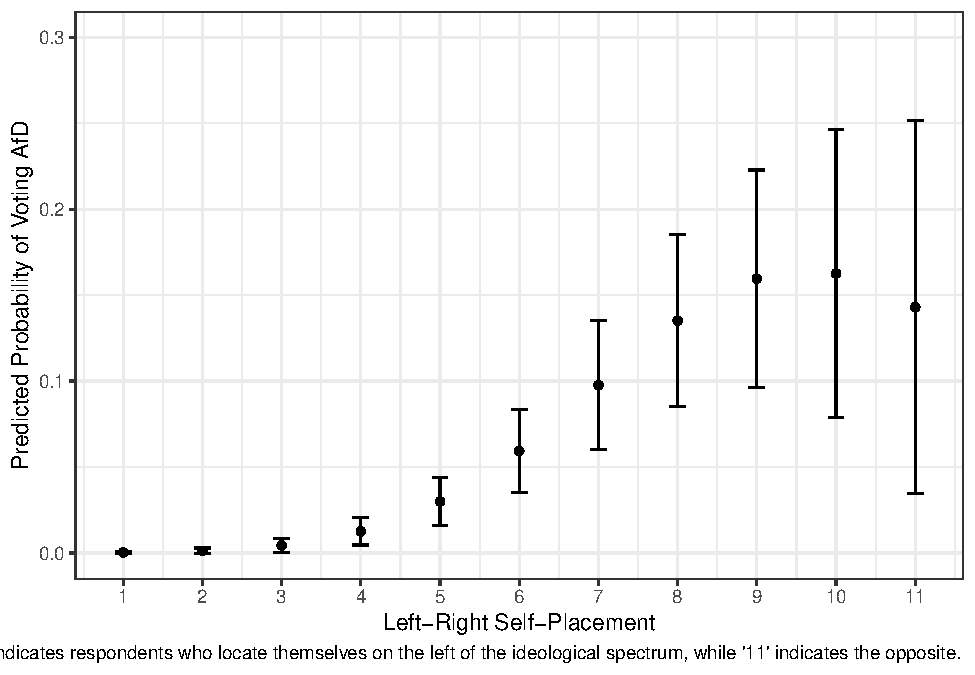
\includegraphics{AVCD_Final_Assignment-Edenhofer_latest_files/figure-latex/afd-left-right-self-placement-1.pdf}

Relationship between age and AfD voting

\begin{Shaded}
\begin{Highlighting}[]
\NormalTok{afd\_age }\OtherTok{\textless{}{-}} \FunctionTok{glm}\NormalTok{(afd\_21 }\SpecialCharTok{\textasciitilde{}}\NormalTok{ age }\SpecialCharTok{+} \FunctionTok{I}\NormalTok{(age}\SpecialCharTok{\^{}}\DecValTok{2}\NormalTok{) }\SpecialCharTok{+}\NormalTok{ household\_income }\SpecialCharTok{+}\NormalTok{ abitur\_factor }\SpecialCharTok{+}\NormalTok{ sex1 }\SpecialCharTok{+}\NormalTok{ urban\_rural\_factor }\SpecialCharTok{+}\NormalTok{ ostwest\_factor, }\AttributeTok{family =} \FunctionTok{binomial}\NormalTok{(}\AttributeTok{link =} \StringTok{"logit"}\NormalTok{), }\AttributeTok{data =}\NormalTok{ gles\_mod)}
\CommentTok{\# plot }
\FunctionTok{cplot}\NormalTok{(afd\_age, }\AttributeTok{x =} \StringTok{"age"}\NormalTok{, }\AttributeTok{draw =}\NormalTok{ F) }\SpecialCharTok{\%\textgreater{}\%}
  \FunctionTok{as\_tibble}\NormalTok{() }\SpecialCharTok{\%\textgreater{}\%}
  \FunctionTok{ggplot}\NormalTok{(}\FunctionTok{aes}\NormalTok{(}\AttributeTok{x =}\NormalTok{ xvals)) }\SpecialCharTok{+}
  \FunctionTok{geom\_line}\NormalTok{(}\FunctionTok{aes}\NormalTok{(}\AttributeTok{y =}\NormalTok{ yvals)) }\SpecialCharTok{+}
  \FunctionTok{geom\_ribbon}\NormalTok{(}\FunctionTok{aes}\NormalTok{(}\AttributeTok{ymin =}\NormalTok{ lower, }\AttributeTok{ymax =}\NormalTok{ upper), }\AttributeTok{alpha =} \FloatTok{0.2}\NormalTok{) }\SpecialCharTok{+}
  \FunctionTok{scale\_x\_continuous}\NormalTok{(}\StringTok{"Age"}\NormalTok{, }\AttributeTok{breaks =} \FunctionTok{seq}\NormalTok{(}\DecValTok{20}\NormalTok{, }\DecValTok{90}\NormalTok{, }\DecValTok{10}\NormalTok{)) }\SpecialCharTok{+}
  \FunctionTok{labs}\NormalTok{(}\AttributeTok{y =} \StringTok{"Predicted Probability of Voting AfD"}\NormalTok{) }\SpecialCharTok{+}
  \FunctionTok{ylim}\NormalTok{(}\FunctionTok{c}\NormalTok{(}\DecValTok{0}\NormalTok{, }\FloatTok{0.15}\NormalTok{)) }\SpecialCharTok{+}
  \FunctionTok{theme\_bw}\NormalTok{()}
\end{Highlighting}
\end{Shaded}

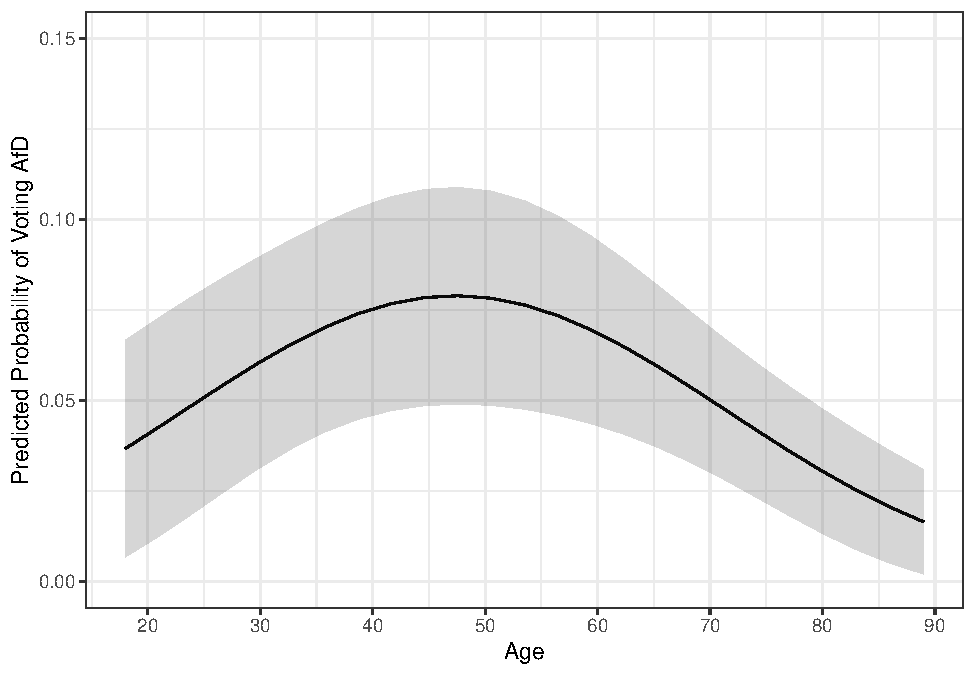
\includegraphics{AVCD_Final_Assignment-Edenhofer_latest_files/figure-latex/afd-age-1.pdf}

Relationship between sex and AfD

\begin{Shaded}
\begin{Highlighting}[]
\FunctionTok{cplot}\NormalTok{(afd\_income, }\AttributeTok{x =} \StringTok{"sex1"}\NormalTok{, }\AttributeTok{draw =}\NormalTok{ F) }\SpecialCharTok{\%\textgreater{}\%}
  \FunctionTok{as\_tibble}\NormalTok{() }\SpecialCharTok{\%\textgreater{}\%}
  \FunctionTok{ggplot}\NormalTok{(}\FunctionTok{aes}\NormalTok{(}\AttributeTok{x =}\NormalTok{ xvals)) }\SpecialCharTok{+}
  \FunctionTok{geom\_point}\NormalTok{(}\FunctionTok{aes}\NormalTok{(}\AttributeTok{y =}\NormalTok{ yvals)) }\SpecialCharTok{+}
  \FunctionTok{geom\_errorbar}\NormalTok{(}\FunctionTok{aes}\NormalTok{(}\AttributeTok{ymin =}\NormalTok{ lower, }\AttributeTok{ymax =}\NormalTok{ upper), }\AttributeTok{width =} \FloatTok{0.2}\NormalTok{) }\SpecialCharTok{+}
  \FunctionTok{scale\_x\_discrete}\NormalTok{(}\StringTok{"Sex"}\NormalTok{, }\AttributeTok{labels =} \FunctionTok{c}\NormalTok{(}\StringTok{"Female"}\NormalTok{, }\StringTok{"Male"}\NormalTok{)) }\SpecialCharTok{+}
  \FunctionTok{ylim}\NormalTok{(}\FunctionTok{c}\NormalTok{(}\DecValTok{0}\NormalTok{, }\FloatTok{0.15}\NormalTok{)) }\SpecialCharTok{+}
  \FunctionTok{labs}\NormalTok{(}\AttributeTok{y =} \StringTok{"Predicted Probability of Voting AfD"}\NormalTok{, }
       \AttributeTok{caption =} \StringTok{"Covariates include: age, household income, education and rurality of place of residence."}\NormalTok{) }\SpecialCharTok{+}
  \FunctionTok{theme\_bw}\NormalTok{()}
\end{Highlighting}
\end{Shaded}

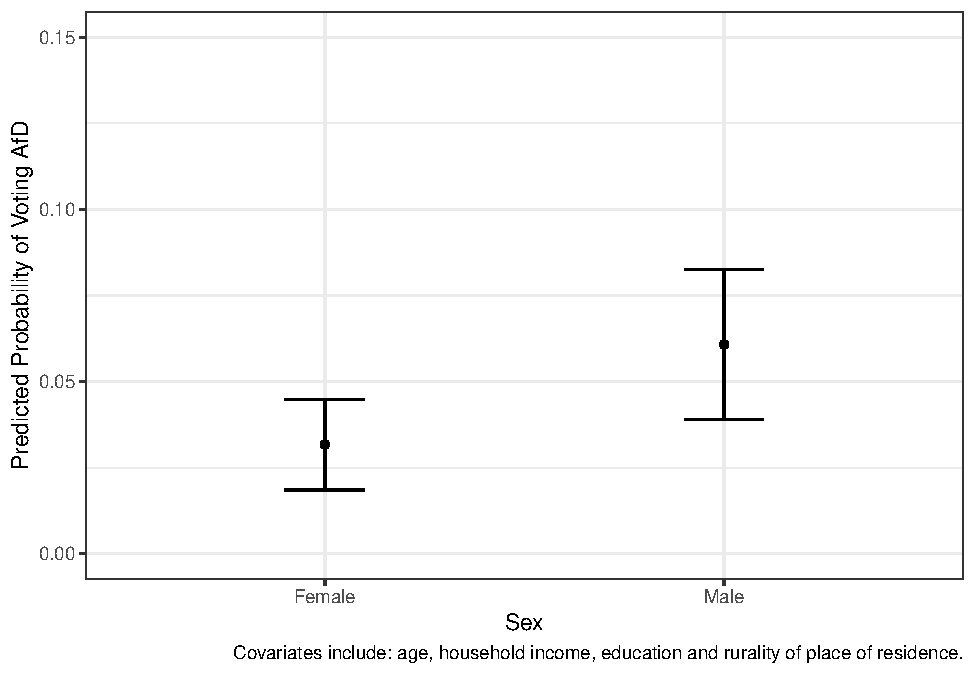
\includegraphics{AVCD_Final_Assignment-Edenhofer_latest_files/figure-latex/afd-sex-1.pdf}

Relationship between education and AfD voting

\begin{Shaded}
\begin{Highlighting}[]
\FunctionTok{cplot}\NormalTok{(afd\_income, }\AttributeTok{x =} \StringTok{"abitur\_factor"}\NormalTok{, }\AttributeTok{draw =}\NormalTok{ F) }\SpecialCharTok{\%\textgreater{}\%}
  \FunctionTok{as\_tibble}\NormalTok{() }\SpecialCharTok{\%\textgreater{}\%}
  \FunctionTok{ggplot}\NormalTok{(}\FunctionTok{aes}\NormalTok{(}\AttributeTok{x =}\NormalTok{ xvals)) }\SpecialCharTok{+}
  \FunctionTok{geom\_point}\NormalTok{(}\FunctionTok{aes}\NormalTok{(}\AttributeTok{y =}\NormalTok{ yvals)) }\SpecialCharTok{+}
  \FunctionTok{geom\_errorbar}\NormalTok{(}\FunctionTok{aes}\NormalTok{(}\AttributeTok{ymin =}\NormalTok{ lower, }\AttributeTok{ymax =}\NormalTok{ upper), }\AttributeTok{width =} \FloatTok{0.2}\NormalTok{) }\SpecialCharTok{+}
  \FunctionTok{scale\_x\_discrete}\NormalTok{(}\StringTok{"Education"}\NormalTok{, }\AttributeTok{labels =} \FunctionTok{c}\NormalTok{(}\StringTok{"At Least Abitur"}\NormalTok{, }
                                           \StringTok{"No Abitur"}\NormalTok{)) }\SpecialCharTok{+}
  \FunctionTok{labs}\NormalTok{(}\AttributeTok{y =} \StringTok{"Predicted Probability of Voting AfD"}\NormalTok{, }
       \AttributeTok{caption =} \StringTok{"Covariates include: age, household income, sex and rurality of place of residence."}\NormalTok{) }\SpecialCharTok{+}
  \FunctionTok{ylim}\NormalTok{(}\FunctionTok{c}\NormalTok{(}\DecValTok{0}\NormalTok{, }\FloatTok{0.15}\NormalTok{)) }\SpecialCharTok{+}
  \FunctionTok{theme\_bw}\NormalTok{()}
\end{Highlighting}
\end{Shaded}

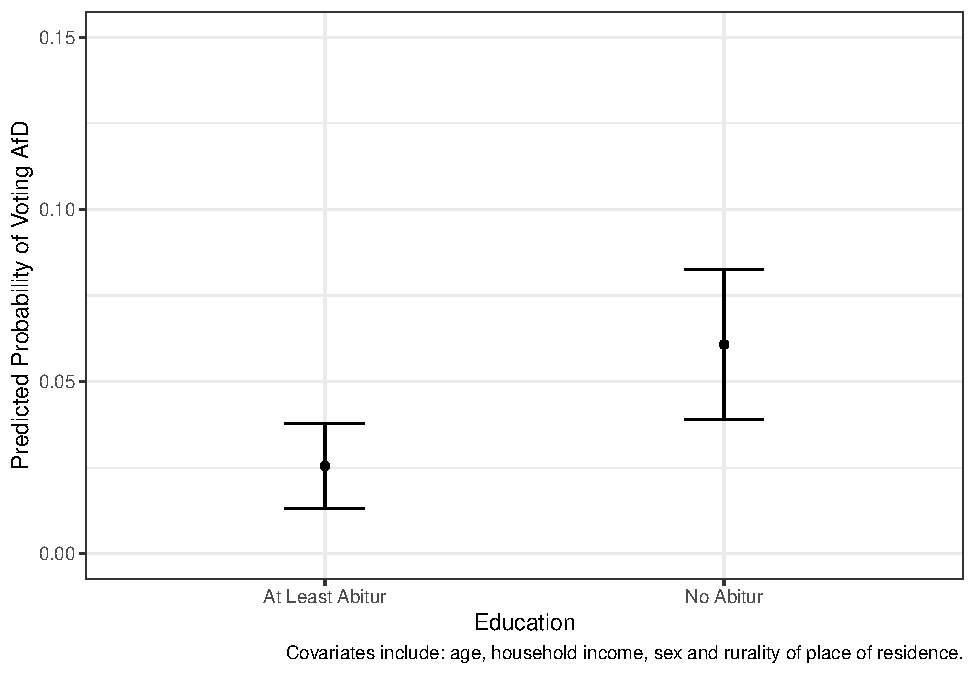
\includegraphics{AVCD_Final_Assignment-Edenhofer_latest_files/figure-latex/afd-education-1.pdf}

\begin{Shaded}
\begin{Highlighting}[]
\FunctionTok{cplot}\NormalTok{(afd\_income, }\AttributeTok{x =} \StringTok{"urban\_rural\_factor"}\NormalTok{, }\AttributeTok{draw =}\NormalTok{ F) }\SpecialCharTok{\%\textgreater{}\%}
  \FunctionTok{as\_tibble}\NormalTok{() }\SpecialCharTok{\%\textgreater{}\%}
  \FunctionTok{ggplot}\NormalTok{(}\FunctionTok{aes}\NormalTok{(}\AttributeTok{x =}\NormalTok{ xvals)) }\SpecialCharTok{+}
  \FunctionTok{geom\_point}\NormalTok{(}\FunctionTok{aes}\NormalTok{(}\AttributeTok{y =}\NormalTok{ yvals)) }\SpecialCharTok{+}
  \FunctionTok{geom\_errorbar}\NormalTok{(}\FunctionTok{aes}\NormalTok{(}\AttributeTok{ymin =}\NormalTok{ lower, }\AttributeTok{ymax =}\NormalTok{ upper), }\AttributeTok{width =} \FloatTok{0.2}\NormalTok{) }\SpecialCharTok{+}
  \FunctionTok{scale\_x\_discrete}\NormalTok{(}\StringTok{"Urban{-}Rural"}\NormalTok{, }
                   \AttributeTok{labels =} \FunctionTok{c}\NormalTok{(}\StringTok{"Grossstadt"}\NormalTok{, }\StringTok{"Rand/Vorort grosser Stadt"}\NormalTok{,}
                              \StringTok{"Mittel{-}oder Kleinstadt"}\NormalTok{, }\StringTok{"laendliches Dorf"}\NormalTok{,}
                              \StringTok{"Einzelgehoeft"}\NormalTok{)) }\SpecialCharTok{+}
 \FunctionTok{labs}\NormalTok{(}\AttributeTok{y =} \StringTok{"Predicted Probability of Voting AfD"}\NormalTok{) }\SpecialCharTok{+}
 \FunctionTok{ylim}\NormalTok{(}\FunctionTok{c}\NormalTok{(}\DecValTok{0}\NormalTok{, }\FloatTok{0.35}\NormalTok{)) }\SpecialCharTok{+}
 \FunctionTok{theme\_bw}\NormalTok{() }\SpecialCharTok{+}
 \FunctionTok{theme}\NormalTok{(}\AttributeTok{axis.text.x =} \FunctionTok{element\_text}\NormalTok{(}\AttributeTok{angle =} \DecValTok{15}\NormalTok{, }\AttributeTok{hjust =} \DecValTok{1}\NormalTok{))}
\end{Highlighting}
\end{Shaded}

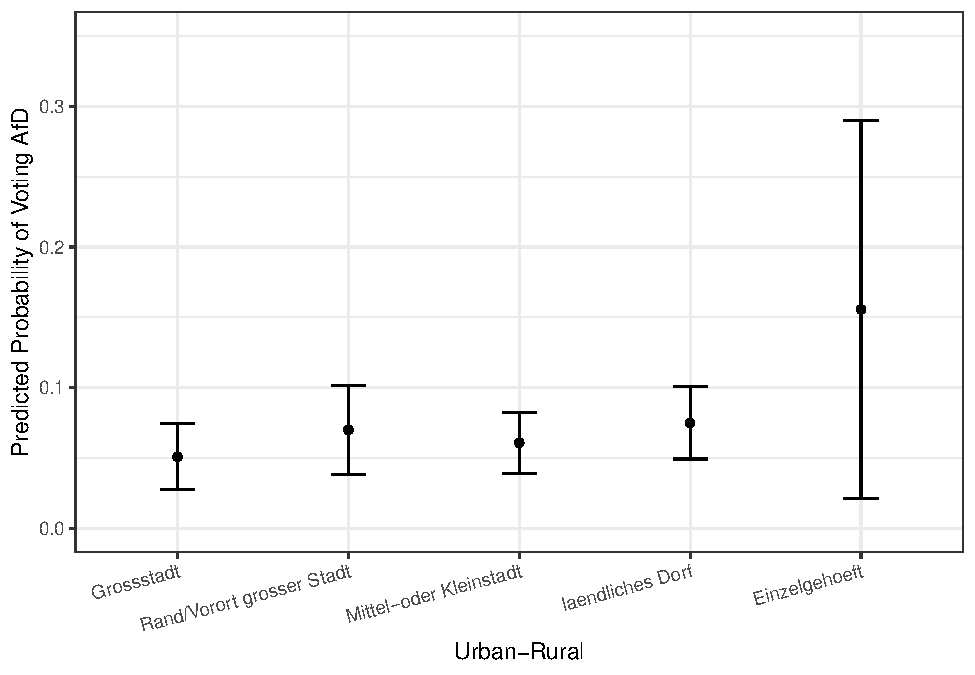
\includegraphics{AVCD_Final_Assignment-Edenhofer_latest_files/figure-latex/afd-geography-1.pdf}

\begin{Shaded}
\begin{Highlighting}[]
\FunctionTok{cplot}\NormalTok{(afd\_income, }\AttributeTok{x =} \StringTok{"ostwest\_factor"}\NormalTok{, }\AttributeTok{draw =}\NormalTok{ F) }\SpecialCharTok{\%\textgreater{}\%}
  \FunctionTok{as\_tibble}\NormalTok{() }\SpecialCharTok{\%\textgreater{}\%}
  \FunctionTok{ggplot}\NormalTok{(}\FunctionTok{aes}\NormalTok{(}\AttributeTok{x =}\NormalTok{ xvals)) }\SpecialCharTok{+}
  \FunctionTok{geom\_point}\NormalTok{(}\FunctionTok{aes}\NormalTok{(}\AttributeTok{y =}\NormalTok{ yvals)) }\SpecialCharTok{+}
  \FunctionTok{geom\_errorbar}\NormalTok{(}\FunctionTok{aes}\NormalTok{(}\AttributeTok{ymin =}\NormalTok{ lower, }\AttributeTok{ymax =}\NormalTok{ upper), }\AttributeTok{width =} \FloatTok{0.2}\NormalTok{) }\SpecialCharTok{+}
  \FunctionTok{scale\_x\_discrete}\NormalTok{(}\StringTok{"Ost{-}West Dummy"}\NormalTok{, }\AttributeTok{labels =} \FunctionTok{c}\NormalTok{(}\StringTok{"Ost"}\NormalTok{, }\StringTok{"West"}\NormalTok{)) }\SpecialCharTok{+}
  \FunctionTok{ylim}\NormalTok{(}\FunctionTok{c}\NormalTok{(}\DecValTok{0}\NormalTok{, }\FloatTok{0.25}\NormalTok{)) }\SpecialCharTok{+}
  \FunctionTok{labs}\NormalTok{(}\AttributeTok{y =} \StringTok{"Predicted Probability of Voting AfD"}\NormalTok{) }\SpecialCharTok{+}
  \FunctionTok{theme\_bw}\NormalTok{()}
\end{Highlighting}
\end{Shaded}

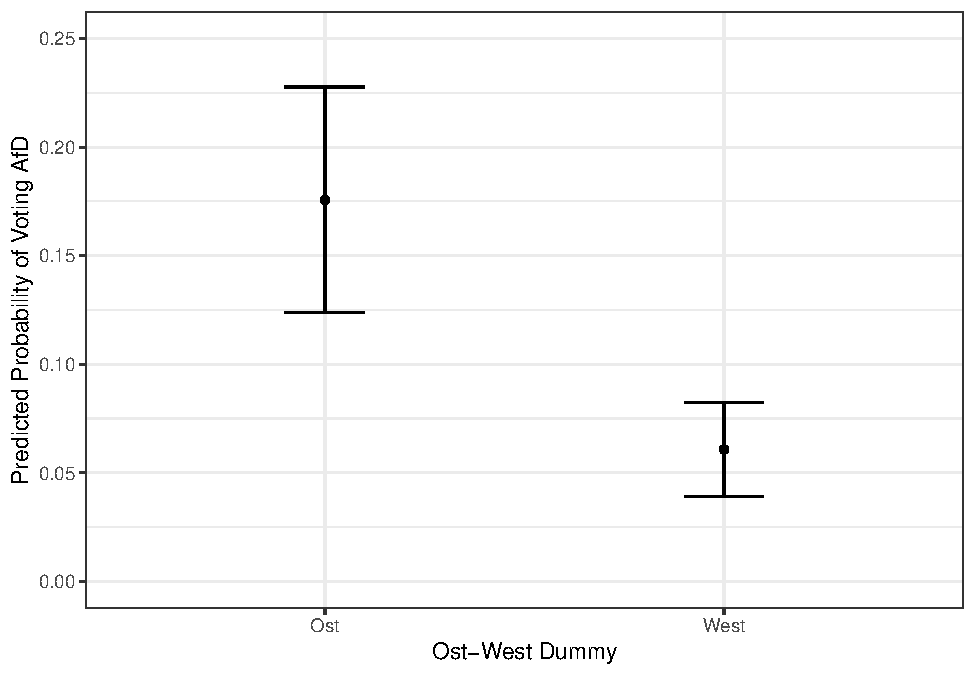
\includegraphics{AVCD_Final_Assignment-Edenhofer_latest_files/figure-latex/afd-ost-west-1.pdf}

\hypertarget{attiudinal-correlates}{%
\subsubsection{Attiudinal Correlates}\label{attiudinal-correlates}}

\begin{Shaded}
\begin{Highlighting}[]
\NormalTok{afd\_cancel\_culture }\OtherTok{\textless{}{-}} \FunctionTok{glm}\NormalTok{(afd\_21 }\SpecialCharTok{\textasciitilde{}}\NormalTok{ cancel\_culture\_subjektiv }\SpecialCharTok{+}\NormalTok{ household\_income }\SpecialCharTok{+}\NormalTok{ age }\SpecialCharTok{+}\NormalTok{ abitur\_factor }\SpecialCharTok{+}\NormalTok{ sex1 }\SpecialCharTok{+}\NormalTok{ urban\_rural\_factor }\SpecialCharTok{+}\NormalTok{ ostwest\_factor, }\AttributeTok{family =} \FunctionTok{binomial}\NormalTok{(}\AttributeTok{link =} \StringTok{"logit"}\NormalTok{), }\AttributeTok{data =}\NormalTok{ gles\_mod)}
\CommentTok{\# plot}
\FunctionTok{cplot}\NormalTok{(afd\_cancel\_culture, }\AttributeTok{x =} \StringTok{"cancel\_culture\_subjektiv"}\NormalTok{, }
      \AttributeTok{xvals =} \FunctionTok{seq}\NormalTok{(}\DecValTok{1}\NormalTok{, }\DecValTok{5}\NormalTok{, }\DecValTok{1}\NormalTok{), }\AttributeTok{draw =}\NormalTok{ F) }\SpecialCharTok{\%\textgreater{}\%}
  \FunctionTok{as\_tibble}\NormalTok{() }\SpecialCharTok{\%\textgreater{}\%}
  \FunctionTok{ggplot}\NormalTok{(}\FunctionTok{aes}\NormalTok{(}\AttributeTok{x =}\NormalTok{ xvals)) }\SpecialCharTok{+}
  \FunctionTok{geom\_point}\NormalTok{(}\FunctionTok{aes}\NormalTok{(}\AttributeTok{y =}\NormalTok{ yvals)) }\SpecialCharTok{+}
  \FunctionTok{geom\_errorbar}\NormalTok{(}\FunctionTok{aes}\NormalTok{(}\AttributeTok{ymin =}\NormalTok{ lower, }\AttributeTok{ymax =}\NormalTok{ upper), }\AttributeTok{width =} \FloatTok{0.2}\NormalTok{) }\SpecialCharTok{+}
  \FunctionTok{scale\_x\_continuous}\NormalTok{(}\StringTok{"Subjektiv: Keine freie Meinungsaeusserung moeglich"}\NormalTok{, }
                   \AttributeTok{breaks =} \FunctionTok{seq}\NormalTok{(}\DecValTok{1}\NormalTok{, }\DecValTok{5}\NormalTok{, }\DecValTok{1}\NormalTok{),}
                   \AttributeTok{labels =} \FunctionTok{c}\NormalTok{(}\StringTok{"Stimme voll zu"}\NormalTok{, }\StringTok{"Stimme eher zu"}\NormalTok{,}
                              \StringTok{"Teils/Teils"}\NormalTok{, }\StringTok{"Stimme eher nicht zu"}\NormalTok{,}
                              \StringTok{"Stimme ueberhaupt nicht zu"}\NormalTok{)) }\SpecialCharTok{+}
  \FunctionTok{labs}\NormalTok{(}\AttributeTok{y =} \StringTok{"Predicted Probability of Voting AfD"}\NormalTok{) }\SpecialCharTok{+}
  \FunctionTok{ylim}\NormalTok{(}\FunctionTok{c}\NormalTok{(}\DecValTok{0}\NormalTok{, }\FloatTok{0.5}\NormalTok{)) }\SpecialCharTok{+}
  \FunctionTok{theme\_bw}\NormalTok{() }\SpecialCharTok{+}
  \FunctionTok{theme}\NormalTok{(}\AttributeTok{axis.text.x =} \FunctionTok{element\_text}\NormalTok{(}\AttributeTok{angle =} \DecValTok{15}\NormalTok{, }\AttributeTok{hjust =} \DecValTok{1}\NormalTok{))}
\end{Highlighting}
\end{Shaded}

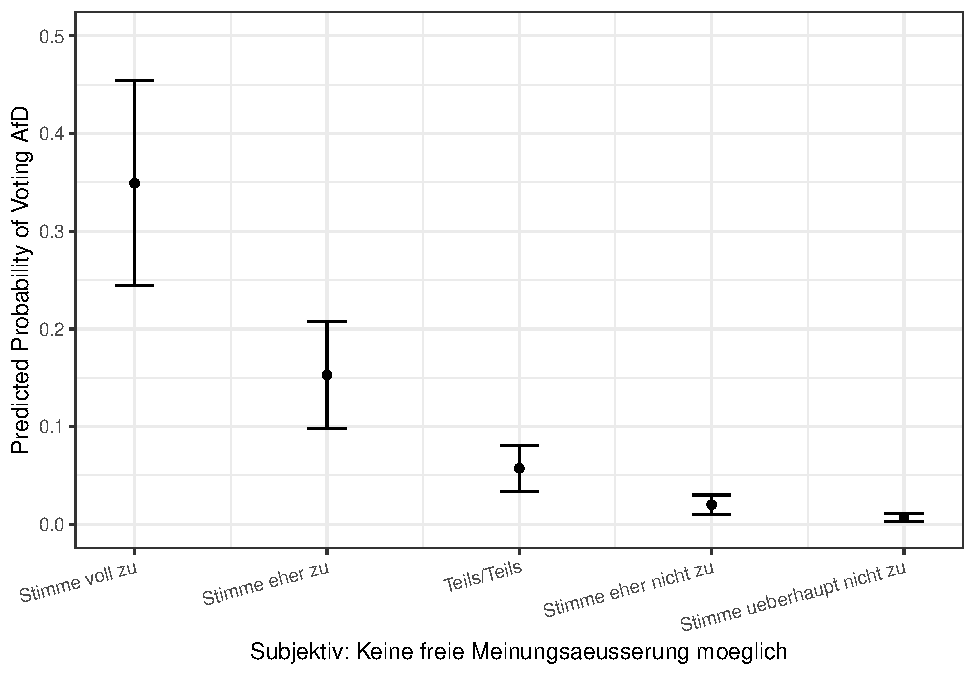
\includegraphics{AVCD_Final_Assignment-Edenhofer_latest_files/figure-latex/afd-cancel-culture-1.pdf}

\begin{Shaded}
\begin{Highlighting}[]
\NormalTok{afd\_trust\_parliament }\OtherTok{\textless{}{-}} \FunctionTok{glm}\NormalTok{(afd\_21 }\SpecialCharTok{\textasciitilde{}}\NormalTok{ trust\_in\_parliament }\SpecialCharTok{+}\NormalTok{ household\_income }\SpecialCharTok{+}\NormalTok{ age }\SpecialCharTok{+}\NormalTok{ abitur\_factor }\SpecialCharTok{+}\NormalTok{ sex1 }\SpecialCharTok{+}\NormalTok{ urban\_rural\_factor }\SpecialCharTok{+}\NormalTok{ ostwest\_factor, }\AttributeTok{family =} \FunctionTok{binomial}\NormalTok{(}\AttributeTok{link =} \StringTok{"logit"}\NormalTok{), }\AttributeTok{data =}\NormalTok{ gles\_mod)}
\CommentTok{\# plot }
\FunctionTok{cplot}\NormalTok{(afd\_trust\_parliament, }\AttributeTok{x =} \StringTok{"trust\_in\_parliament"}\NormalTok{,}
      \AttributeTok{xvals =} \FunctionTok{seq}\NormalTok{(}\DecValTok{1}\NormalTok{, }\DecValTok{11}\NormalTok{, }\DecValTok{1}\NormalTok{), }\AttributeTok{draw =}\NormalTok{ F)  }\SpecialCharTok{\%\textgreater{}\%}
  \FunctionTok{as\_tibble}\NormalTok{() }\SpecialCharTok{\%\textgreater{}\%}
  \FunctionTok{ggplot}\NormalTok{(}\FunctionTok{aes}\NormalTok{(}\AttributeTok{x =}\NormalTok{ xvals)) }\SpecialCharTok{+}
  \FunctionTok{geom\_point}\NormalTok{(}\FunctionTok{aes}\NormalTok{(}\AttributeTok{y =}\NormalTok{ yvals)) }\SpecialCharTok{+}
  \FunctionTok{geom\_errorbar}\NormalTok{(}\FunctionTok{aes}\NormalTok{(}\AttributeTok{ymin =}\NormalTok{ lower, }\AttributeTok{ymax =}\NormalTok{ upper), }\AttributeTok{width =} \FloatTok{0.2}\NormalTok{) }\SpecialCharTok{+}
  \FunctionTok{scale\_x\_continuous}\NormalTok{(}\StringTok{"Vertrauen: Bundestag"}\NormalTok{, }
                     \AttributeTok{breaks =} \FunctionTok{seq}\NormalTok{(}\DecValTok{1}\NormalTok{, }\DecValTok{11}\NormalTok{, }\DecValTok{1}\NormalTok{)) }\SpecialCharTok{+}
  \FunctionTok{labs}\NormalTok{(}\AttributeTok{y =} \StringTok{"Predicted Probability of Voting AfD"}\NormalTok{, }
       \AttributeTok{caption =} \StringTok{"\textquotesingle{}1\textquotesingle{} indicates \textquotesingle{}no trust\textquotesingle{}, while 11 indicates \textquotesingle{}full trust\textquotesingle{}."}\NormalTok{) }\SpecialCharTok{+}
  \FunctionTok{ylim}\NormalTok{(}\FunctionTok{c}\NormalTok{(}\DecValTok{0}\NormalTok{, }\FloatTok{0.6}\NormalTok{)) }\SpecialCharTok{+}
  \FunctionTok{theme\_bw}\NormalTok{()}
\end{Highlighting}
\end{Shaded}

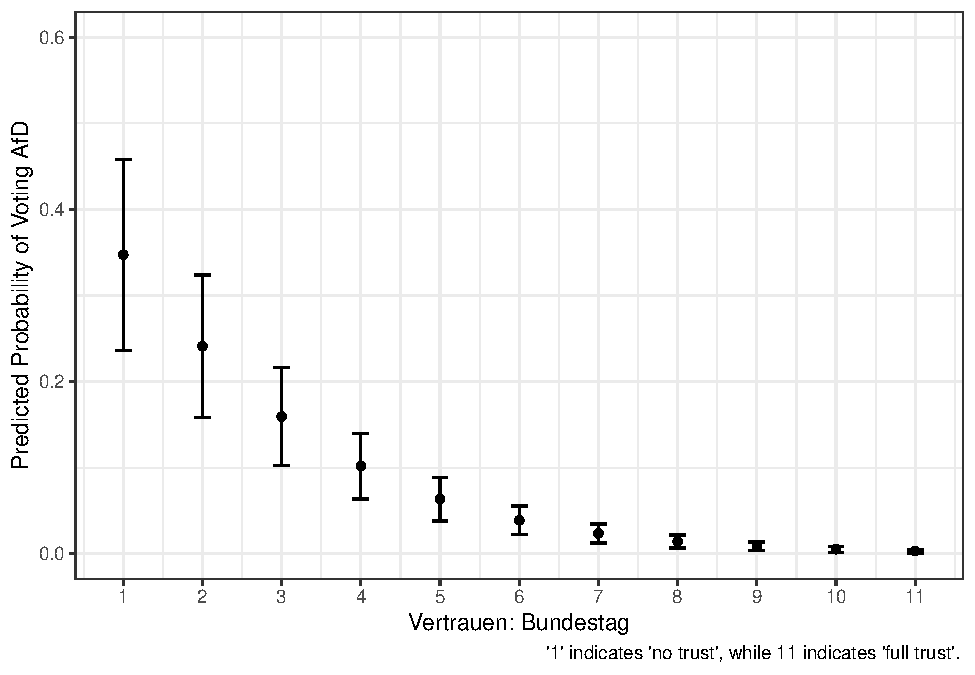
\includegraphics{AVCD_Final_Assignment-Edenhofer_latest_files/figure-latex/afd-trust-parliament-1.pdf}

\begin{Shaded}
\begin{Highlighting}[]
\NormalTok{afd\_trust\_parties }\OtherTok{\textless{}{-}} \FunctionTok{glm}\NormalTok{(afd\_21 }\SpecialCharTok{\textasciitilde{}}\NormalTok{ trust\_in\_parties }\SpecialCharTok{+}\NormalTok{ household\_income }\SpecialCharTok{+}\NormalTok{ age }\SpecialCharTok{+}\NormalTok{ abitur\_factor }\SpecialCharTok{+}\NormalTok{ sex1 }\SpecialCharTok{+}\NormalTok{ urban\_rural\_factor }\SpecialCharTok{+}\NormalTok{ ostwest\_factor, }\AttributeTok{family =} \FunctionTok{binomial}\NormalTok{(}\AttributeTok{link =} \StringTok{"logit"}\NormalTok{), }\AttributeTok{data =}\NormalTok{ gles\_mod)}
\CommentTok{\# plot }
\FunctionTok{cplot}\NormalTok{(afd\_trust\_parties, }\AttributeTok{x =} \StringTok{"trust\_in\_parties"}\NormalTok{,}
      \AttributeTok{xvals =} \FunctionTok{seq}\NormalTok{(}\DecValTok{1}\NormalTok{, }\DecValTok{11}\NormalTok{, }\DecValTok{1}\NormalTok{), }\AttributeTok{draw =}\NormalTok{ F) }\SpecialCharTok{\%\textgreater{}\%}
  \FunctionTok{as\_tibble}\NormalTok{() }\SpecialCharTok{\%\textgreater{}\%}
  \FunctionTok{ggplot}\NormalTok{(}\FunctionTok{aes}\NormalTok{(}\AttributeTok{x =}\NormalTok{ xvals)) }\SpecialCharTok{+}
  \FunctionTok{geom\_point}\NormalTok{(}\FunctionTok{aes}\NormalTok{(}\AttributeTok{y =}\NormalTok{ yvals)) }\SpecialCharTok{+}
  \FunctionTok{geom\_errorbar}\NormalTok{(}\FunctionTok{aes}\NormalTok{(}\AttributeTok{ymin =}\NormalTok{ lower, }\AttributeTok{ymax =}\NormalTok{ upper), }\AttributeTok{width =} \FloatTok{0.2}\NormalTok{) }\SpecialCharTok{+}
  \FunctionTok{scale\_x\_continuous}\NormalTok{(}\StringTok{"Vertrauen: Parteien"}\NormalTok{, }
                     \AttributeTok{breaks =} \FunctionTok{seq}\NormalTok{(}\DecValTok{1}\NormalTok{, }\DecValTok{11}\NormalTok{, }\DecValTok{1}\NormalTok{)) }\SpecialCharTok{+}
  \FunctionTok{labs}\NormalTok{(}\AttributeTok{y =} \StringTok{"Predicted Probability of Voting AfD"}\NormalTok{, }
       \AttributeTok{caption =} \StringTok{"\textquotesingle{}1\textquotesingle{} indicates \textquotesingle{}no trust\textquotesingle{}, while 11 indicates \textquotesingle{}full trust\textquotesingle{}."}\NormalTok{) }\SpecialCharTok{+}
  \FunctionTok{ylim}\NormalTok{(}\FunctionTok{c}\NormalTok{(}\DecValTok{0}\NormalTok{, }\FloatTok{0.6}\NormalTok{)) }\SpecialCharTok{+}
  \FunctionTok{theme\_bw}\NormalTok{()}
\end{Highlighting}
\end{Shaded}

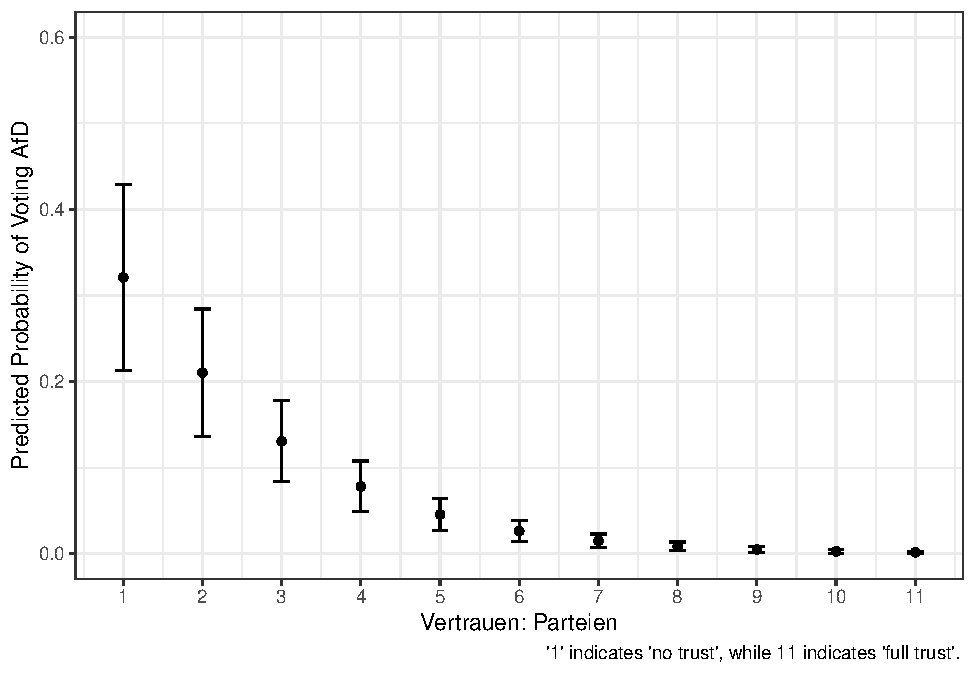
\includegraphics{AVCD_Final_Assignment-Edenhofer_latest_files/figure-latex/afd-trust-parties-1.pdf}

\begin{Shaded}
\begin{Highlighting}[]
\NormalTok{afd\_trust\_politicians }\OtherTok{\textless{}{-}} \FunctionTok{glm}\NormalTok{(afd\_21 }\SpecialCharTok{\textasciitilde{}}\NormalTok{ trust\_in\_politicians }\SpecialCharTok{+}\NormalTok{ household\_income }\SpecialCharTok{+}\NormalTok{ age }\SpecialCharTok{+}\NormalTok{ abitur\_factor }\SpecialCharTok{+}\NormalTok{ sex1 }\SpecialCharTok{+}\NormalTok{ urban\_rural\_factor }\SpecialCharTok{+}\NormalTok{ ostwest\_factor, }\AttributeTok{family =} \FunctionTok{binomial}\NormalTok{(}\AttributeTok{link =} \StringTok{"logit"}\NormalTok{), }\AttributeTok{data =}\NormalTok{ gles\_mod)}
\CommentTok{\# plot }
\FunctionTok{cplot}\NormalTok{(afd\_trust\_politicians, }\AttributeTok{x =} \StringTok{"trust\_in\_politicians"}\NormalTok{,}
      \AttributeTok{xvals =} \FunctionTok{seq}\NormalTok{(}\DecValTok{1}\NormalTok{, }\DecValTok{11}\NormalTok{, }\DecValTok{1}\NormalTok{), }\AttributeTok{draw =}\NormalTok{ F)  }\SpecialCharTok{\%\textgreater{}\%}
  \FunctionTok{as\_tibble}\NormalTok{() }\SpecialCharTok{\%\textgreater{}\%}
  \FunctionTok{ggplot}\NormalTok{(}\FunctionTok{aes}\NormalTok{(}\AttributeTok{x =}\NormalTok{ xvals)) }\SpecialCharTok{+}
  \FunctionTok{geom\_point}\NormalTok{(}\FunctionTok{aes}\NormalTok{(}\AttributeTok{y =}\NormalTok{ yvals)) }\SpecialCharTok{+}
  \FunctionTok{geom\_errorbar}\NormalTok{(}\FunctionTok{aes}\NormalTok{(}\AttributeTok{ymin =}\NormalTok{ lower, }\AttributeTok{ymax =}\NormalTok{ upper), }\AttributeTok{width =} \FloatTok{0.2}\NormalTok{) }\SpecialCharTok{+}
  \FunctionTok{scale\_x\_continuous}\NormalTok{(}\StringTok{"Vertrauen: Politiker:innen"}\NormalTok{, }
                     \AttributeTok{breaks =} \FunctionTok{seq}\NormalTok{(}\DecValTok{1}\NormalTok{, }\DecValTok{11}\NormalTok{, }\DecValTok{1}\NormalTok{)) }\SpecialCharTok{+}
  \FunctionTok{labs}\NormalTok{(}\AttributeTok{y =} \StringTok{"Predicted Probability of Voting AfD"}\NormalTok{, }
       \AttributeTok{caption =} \StringTok{"\textquotesingle{}1\textquotesingle{} indicates \textquotesingle{}no trust\textquotesingle{}, while 11 indicates \textquotesingle{}full trust\textquotesingle{}."}\NormalTok{) }\SpecialCharTok{+}
  \FunctionTok{ylim}\NormalTok{(}\FunctionTok{c}\NormalTok{(}\DecValTok{0}\NormalTok{, }\FloatTok{0.5}\NormalTok{)) }\SpecialCharTok{+}
  \FunctionTok{theme\_bw}\NormalTok{()}
\end{Highlighting}
\end{Shaded}

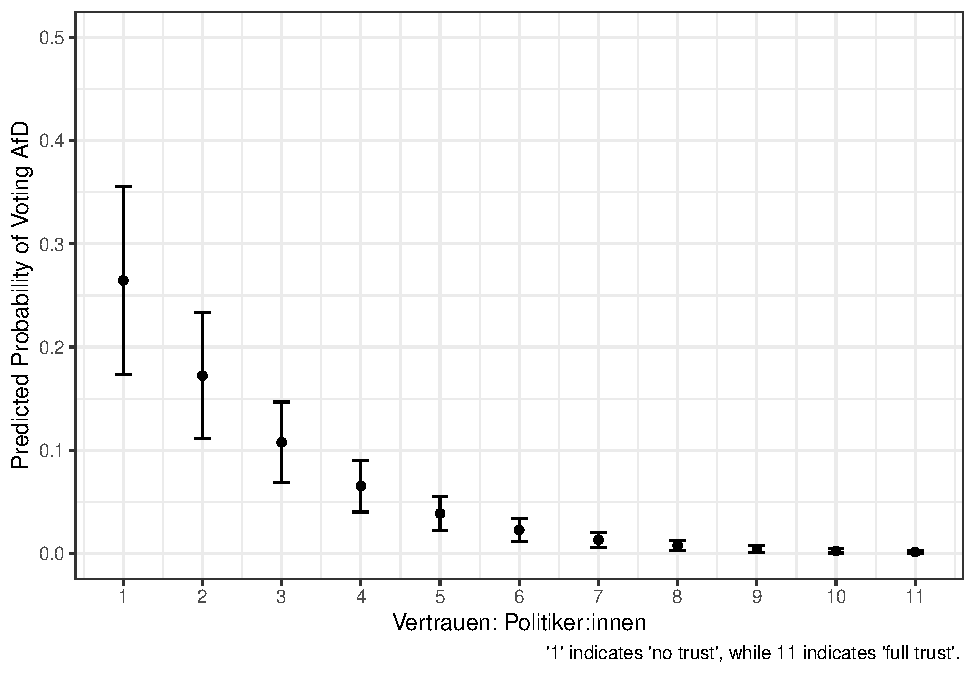
\includegraphics{AVCD_Final_Assignment-Edenhofer_latest_files/figure-latex/afd-trust-politicians-1.pdf}

\begin{Shaded}
\begin{Highlighting}[]
\NormalTok{afd\_trust\_unemp\_politicians }\OtherTok{\textless{}{-}} \FunctionTok{glm}\NormalTok{(afd\_21 }\SpecialCharTok{\textasciitilde{}}\NormalTok{ trust\_in\_politicians}\SpecialCharTok{*}\NormalTok{econ\_current\_personal }\SpecialCharTok{+}\NormalTok{ household\_income }\SpecialCharTok{+}\NormalTok{ age }\SpecialCharTok{+}\NormalTok{ abitur\_factor }\SpecialCharTok{+}\NormalTok{ sex1 }\SpecialCharTok{+}\NormalTok{ urban\_rural\_factor }\SpecialCharTok{+}\NormalTok{ ostwest\_factor, }\AttributeTok{family =} \FunctionTok{binomial}\NormalTok{(}\AttributeTok{link =} \StringTok{"logit"}\NormalTok{), }\AttributeTok{data =}\NormalTok{ gles\_mod)}

\FunctionTok{modelplot}\NormalTok{(afd\_trust\_unemp\_politicians) }\SpecialCharTok{+}
  \FunctionTok{geom\_vline}\NormalTok{(}\AttributeTok{xintercept =} \DecValTok{0}\NormalTok{, }\AttributeTok{linetype =} \StringTok{"dashed"}\NormalTok{)}
\end{Highlighting}
\end{Shaded}

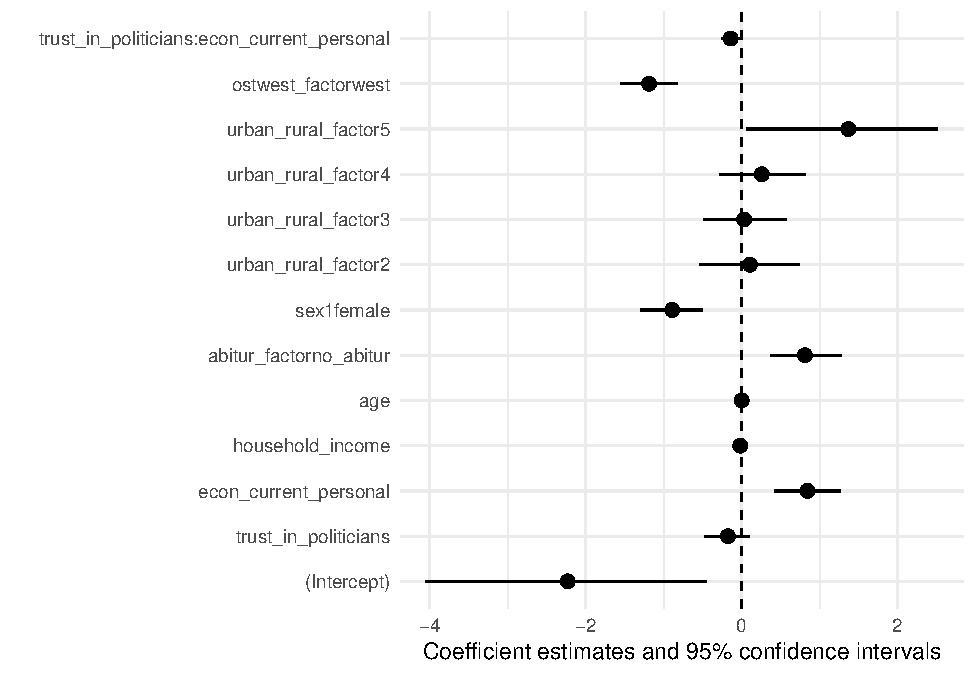
\includegraphics{AVCD_Final_Assignment-Edenhofer_latest_files/figure-latex/unnamed-chunk-1-1.pdf}

\begin{Shaded}
\begin{Highlighting}[]
\NormalTok{afd\_immig\_culture\_threat }\OtherTok{\textless{}{-}} \FunctionTok{glm}\NormalTok{(afd\_21 }\SpecialCharTok{\textasciitilde{}}\NormalTok{ out\_group\_immig\_culture\_threat }\SpecialCharTok{+}\NormalTok{ household\_income }\SpecialCharTok{+}\NormalTok{ age }\SpecialCharTok{+}\NormalTok{ abitur\_factor }\SpecialCharTok{+}\NormalTok{ sex1 }\SpecialCharTok{+}\NormalTok{ urban\_rural\_factor }\SpecialCharTok{+}\NormalTok{ ostwest\_factor, }\AttributeTok{family =} \FunctionTok{binomial}\NormalTok{(}\AttributeTok{link =} \StringTok{"logit"}\NormalTok{), }\AttributeTok{data =}\NormalTok{ gles\_mod)}
\CommentTok{\# plot }
\FunctionTok{cplot}\NormalTok{(afd\_immig\_culture\_threat, }\AttributeTok{x =} \StringTok{"out\_group\_immig\_culture\_threat"}\NormalTok{,}
      \AttributeTok{xvals =} \FunctionTok{seq}\NormalTok{(}\DecValTok{1}\NormalTok{, }\DecValTok{5}\NormalTok{, }\DecValTok{1}\NormalTok{), }\AttributeTok{draw =}\NormalTok{ F) }\SpecialCharTok{\%\textgreater{}\%}
  \FunctionTok{as\_tibble}\NormalTok{() }\SpecialCharTok{\%\textgreater{}\%}
  \FunctionTok{ggplot}\NormalTok{(}\FunctionTok{aes}\NormalTok{(}\AttributeTok{x =}\NormalTok{ xvals)) }\SpecialCharTok{+}
  \FunctionTok{geom\_point}\NormalTok{(}\FunctionTok{aes}\NormalTok{(}\AttributeTok{y =}\NormalTok{ yvals)) }\SpecialCharTok{+}
  \FunctionTok{geom\_errorbar}\NormalTok{(}\FunctionTok{aes}\NormalTok{(}\AttributeTok{ymin =}\NormalTok{ lower, }\AttributeTok{ymax =}\NormalTok{ upper), }\AttributeTok{width =} \FloatTok{0.2}\NormalTok{) }\SpecialCharTok{+}
  \FunctionTok{scale\_x\_continuous}\NormalTok{(}\StringTok{"Deutsche Kultur durch Immigration bedroht"}\NormalTok{, }
                     \AttributeTok{breaks =} \FunctionTok{seq}\NormalTok{(}\DecValTok{1}\NormalTok{, }\DecValTok{5}\NormalTok{, }\DecValTok{1}\NormalTok{), }
                     \AttributeTok{labels =} \FunctionTok{c}\NormalTok{(}\StringTok{"Stimme voll und ganz zu"}\NormalTok{, }\StringTok{"Stimme eher zu"}\NormalTok{, }
                                \StringTok{"Teils/Teils"}\NormalTok{, }\StringTok{"Lehne eher ab"}\NormalTok{, }
                                \StringTok{"Lehne voll und ganz ab"}\NormalTok{)) }\SpecialCharTok{+}
  \FunctionTok{labs}\NormalTok{(}\AttributeTok{y =} \StringTok{"Predicted Probability of Voting AfD"}\NormalTok{) }\SpecialCharTok{+}
  \FunctionTok{ylim}\NormalTok{(}\DecValTok{0}\NormalTok{, }\FloatTok{0.5}\NormalTok{) }\SpecialCharTok{+}
  \FunctionTok{theme\_bw}\NormalTok{() }
\end{Highlighting}
\end{Shaded}

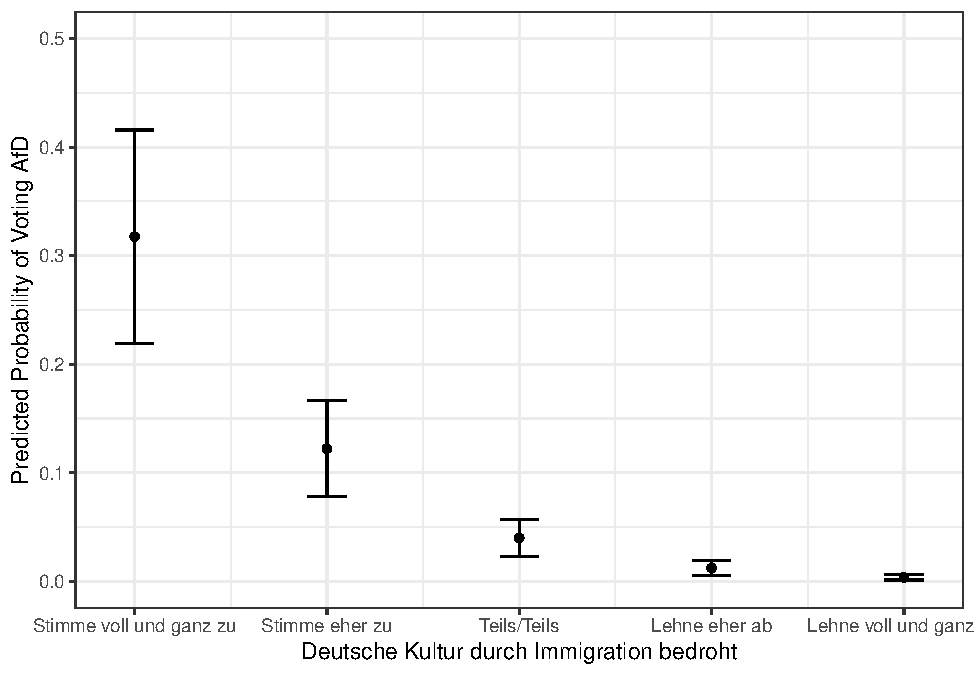
\includegraphics{AVCD_Final_Assignment-Edenhofer_latest_files/figure-latex/afd-immig-culture-threat-1.pdf}

\begin{Shaded}
\begin{Highlighting}[]
\NormalTok{afd\_immig\_crime }\OtherTok{\textless{}{-}} \FunctionTok{glm}\NormalTok{(afd\_21 }\SpecialCharTok{\textasciitilde{}}\NormalTok{ out\_group\_immig\_crime }\SpecialCharTok{+}\NormalTok{ household\_income }\SpecialCharTok{+}\NormalTok{ age }\SpecialCharTok{+}\NormalTok{ abitur\_factor }\SpecialCharTok{+}\NormalTok{ sex1 }\SpecialCharTok{+}\NormalTok{ urban\_rural\_factor }\SpecialCharTok{+}\NormalTok{ ostwest\_factor, }\AttributeTok{family =} \FunctionTok{binomial}\NormalTok{(}\AttributeTok{link =} \StringTok{"logit"}\NormalTok{), }\AttributeTok{data =}\NormalTok{ gles\_mod)}
\CommentTok{\# plot }
\FunctionTok{cplot}\NormalTok{(afd\_immig\_crime, }\AttributeTok{x =} \StringTok{"out\_group\_immig\_crime"}\NormalTok{,}
      \AttributeTok{xvals =} \FunctionTok{seq}\NormalTok{(}\DecValTok{1}\NormalTok{, }\DecValTok{5}\NormalTok{, }\DecValTok{1}\NormalTok{), }\AttributeTok{draw =}\NormalTok{ F) }\SpecialCharTok{\%\textgreater{}\%}
  \FunctionTok{as\_tibble}\NormalTok{() }\SpecialCharTok{\%\textgreater{}\%}
  \FunctionTok{ggplot}\NormalTok{(}\FunctionTok{aes}\NormalTok{(}\AttributeTok{x =}\NormalTok{ xvals)) }\SpecialCharTok{+}
  \FunctionTok{geom\_point}\NormalTok{(}\FunctionTok{aes}\NormalTok{(}\AttributeTok{y =}\NormalTok{ yvals)) }\SpecialCharTok{+}
  \FunctionTok{geom\_errorbar}\NormalTok{(}\FunctionTok{aes}\NormalTok{(}\AttributeTok{ymin =}\NormalTok{ lower, }\AttributeTok{ymax =}\NormalTok{ upper), }\AttributeTok{width =} \FloatTok{0.2}\NormalTok{) }\SpecialCharTok{+}
  \FunctionTok{scale\_x\_continuous}\NormalTok{(}\StringTok{"Immigration erhoeht Kriminalitaet in BRD"}\NormalTok{, }
                     \AttributeTok{breaks =} \FunctionTok{seq}\NormalTok{(}\DecValTok{1}\NormalTok{, }\DecValTok{5}\NormalTok{, }\DecValTok{1}\NormalTok{), }
                     \AttributeTok{labels =} \FunctionTok{c}\NormalTok{(}\StringTok{"Stimme voll und ganz zu"}\NormalTok{, }\StringTok{"Stimme eher zu"}\NormalTok{, }
                                \StringTok{"Teils/Teils"}\NormalTok{, }\StringTok{"Lehne eher ab"}\NormalTok{, }
                                \StringTok{"Lehne voll und ganz ab"}\NormalTok{)) }\SpecialCharTok{+}
  \FunctionTok{labs}\NormalTok{(}\AttributeTok{y =} \StringTok{"Predicted Probability of Voting AfD"}\NormalTok{) }\SpecialCharTok{+}
  \FunctionTok{ylim}\NormalTok{(}\FunctionTok{c}\NormalTok{(}\DecValTok{0}\NormalTok{, }\FloatTok{0.4}\NormalTok{)) }\SpecialCharTok{+}
  \FunctionTok{theme\_bw}\NormalTok{() }
\end{Highlighting}
\end{Shaded}

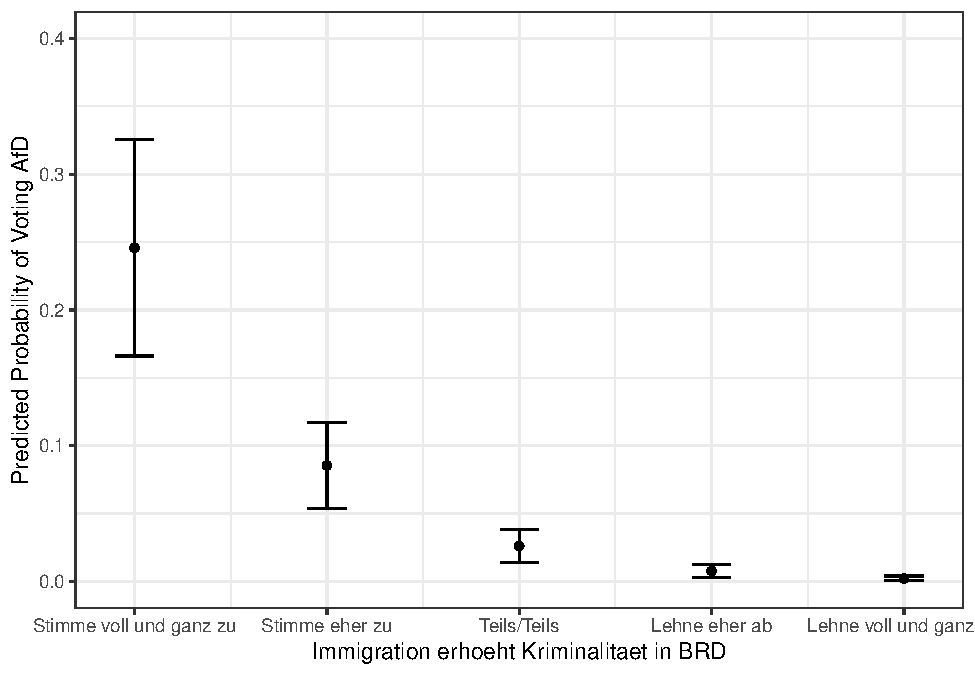
\includegraphics{AVCD_Final_Assignment-Edenhofer_latest_files/figure-latex/afd-immig-crime-1.pdf}

\begin{Shaded}
\begin{Highlighting}[]
\NormalTok{afd\_majority\_will }\OtherTok{\textless{}{-}} \FunctionTok{glm}\NormalTok{(afd\_21 }\SpecialCharTok{\textasciitilde{}}\NormalTok{ out\_group\_majority\_will }\SpecialCharTok{+}\NormalTok{ household\_income }\SpecialCharTok{+}\NormalTok{ age }\SpecialCharTok{+}\NormalTok{ abitur\_factor }\SpecialCharTok{+}\NormalTok{ sex1 }\SpecialCharTok{+}\NormalTok{ urban\_rural\_factor }\SpecialCharTok{+}\NormalTok{ ostwest\_factor, }\AttributeTok{family =} \FunctionTok{binomial}\NormalTok{(}\AttributeTok{link =} \StringTok{"logit"}\NormalTok{), }\AttributeTok{data =}\NormalTok{ gles\_mod)}
\CommentTok{\# plot }
\FunctionTok{cplot}\NormalTok{(afd\_majority\_will, }\AttributeTok{x =} \StringTok{"out\_group\_majority\_will"}\NormalTok{, }
      \AttributeTok{xvals =} \FunctionTok{seq}\NormalTok{(}\DecValTok{1}\NormalTok{, }\DecValTok{5}\NormalTok{, }\DecValTok{1}\NormalTok{), }\AttributeTok{draw =}\NormalTok{ F) }\SpecialCharTok{\%\textgreater{}\%}
  \FunctionTok{as\_tibble}\NormalTok{() }\SpecialCharTok{\%\textgreater{}\%}
  \FunctionTok{ggplot}\NormalTok{(}\FunctionTok{aes}\NormalTok{(}\AttributeTok{x =}\NormalTok{ xvals)) }\SpecialCharTok{+}
  \FunctionTok{geom\_point}\NormalTok{(}\FunctionTok{aes}\NormalTok{(}\AttributeTok{y =}\NormalTok{ yvals)) }\SpecialCharTok{+}
  \FunctionTok{geom\_errorbar}\NormalTok{(}\FunctionTok{aes}\NormalTok{(}\AttributeTok{ymin =}\NormalTok{ lower, }\AttributeTok{ymax =}\NormalTok{ upper), }\AttributeTok{width =} \FloatTok{0.2}\NormalTok{) }\SpecialCharTok{+}
  \FunctionTok{scale\_x\_continuous}\NormalTok{(}\StringTok{"Wille der Mehrheit hat Vorrang"}\NormalTok{, }
                     \AttributeTok{breaks =} \FunctionTok{seq}\NormalTok{(}\DecValTok{1}\NormalTok{, }\DecValTok{5}\NormalTok{, }\DecValTok{1}\NormalTok{),}
                     \AttributeTok{labels =} \FunctionTok{c}\NormalTok{(}\StringTok{"Stimme voll und ganz zu"}\NormalTok{, }\StringTok{"Stimme eher zu"}\NormalTok{, }
                                \StringTok{"Teils/Teils"}\NormalTok{, }\StringTok{"Lehne eher ab"}\NormalTok{, }
                                \StringTok{"Lehne voll und ganz ab"}\NormalTok{)) }\SpecialCharTok{+}
  \FunctionTok{ylim}\NormalTok{(}\FunctionTok{c}\NormalTok{(}\DecValTok{0}\NormalTok{, }\FloatTok{0.2}\NormalTok{)) }\SpecialCharTok{+}
  \FunctionTok{labs}\NormalTok{(}\AttributeTok{y =} \StringTok{"Predicted Probability of Voting AfD"}\NormalTok{) }\SpecialCharTok{+}
  \FunctionTok{theme\_bw}\NormalTok{()}
\end{Highlighting}
\end{Shaded}

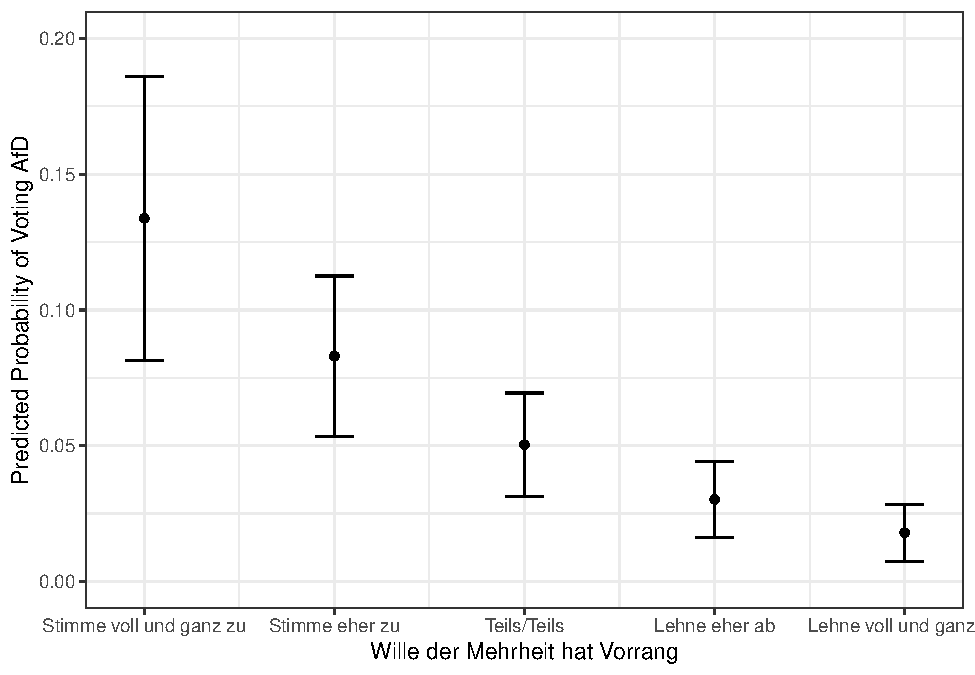
\includegraphics{AVCD_Final_Assignment-Edenhofer_latest_files/figure-latex/afd-majority-will-1.pdf}

\begin{Shaded}
\begin{Highlighting}[]
\NormalTok{afd\_gender1 }\OtherTok{\textless{}{-}} \FunctionTok{glm}\NormalTok{(afd\_21 }\SpecialCharTok{\textasciitilde{}}\NormalTok{ gender\_too\_far }\SpecialCharTok{+}\NormalTok{ age }\SpecialCharTok{+}\NormalTok{ abitur\_factor }\SpecialCharTok{+}\NormalTok{ sex1 }\SpecialCharTok{+}\NormalTok{ urban\_rural\_factor }\SpecialCharTok{+}\NormalTok{ ostwest\_factor, }
                  \AttributeTok{family =} \FunctionTok{binomial}\NormalTok{(}\AttributeTok{link =} \StringTok{"logit"}\NormalTok{), }
                  \AttributeTok{data =}\NormalTok{ gles\_mod)}
\NormalTok{afd\_gender2 }\OtherTok{\textless{}{-}} \FunctionTok{glm}\NormalTok{(afd\_21 }\SpecialCharTok{\textasciitilde{}}\NormalTok{ gender\_too\_far }\SpecialCharTok{+}\NormalTok{ unemployed\_dummy }\SpecialCharTok{+}\NormalTok{ sex1 }\SpecialCharTok{+}\NormalTok{ age }\SpecialCharTok{+}\NormalTok{ abitur\_factor }\SpecialCharTok{+}\NormalTok{  urban\_rural\_factor }\SpecialCharTok{+}\NormalTok{ ostwest\_factor, }
                  \AttributeTok{family =} \FunctionTok{binomial}\NormalTok{(}\AttributeTok{link =} \StringTok{"logit"}\NormalTok{), }
                  \AttributeTok{data =}\NormalTok{ gles\_mod)}
\NormalTok{afd\_gender3 }\OtherTok{\textless{}{-}} \FunctionTok{glm}\NormalTok{(afd\_21 }\SpecialCharTok{\textasciitilde{}}\NormalTok{ gender\_too\_far}\SpecialCharTok{*}\NormalTok{econ\_current\_personal }\SpecialCharTok{+}\NormalTok{ abitur\_factor }\SpecialCharTok{+}\NormalTok{ sex1 }\SpecialCharTok{+}\NormalTok{ age }\SpecialCharTok{+}\NormalTok{ abitur\_factor }\SpecialCharTok{+}\NormalTok{  urban\_rural\_factor }\SpecialCharTok{+}\NormalTok{ ostwest\_factor, }
                  \AttributeTok{family =} \FunctionTok{binomial}\NormalTok{(}\AttributeTok{link =} \StringTok{"logit"}\NormalTok{), }
                  \AttributeTok{data =}\NormalTok{ gles\_mod)}
\NormalTok{afd\_gender4 }\OtherTok{\textless{}{-}} \FunctionTok{glm}\NormalTok{(afd\_21 }\SpecialCharTok{\textasciitilde{}}\NormalTok{ gender\_too\_far}\SpecialCharTok{*}\NormalTok{econ\_personal\_gov\_resp }\SpecialCharTok{+}\NormalTok{ abitur\_factor }\SpecialCharTok{+}\NormalTok{ sex1 }\SpecialCharTok{+}\NormalTok{ age }\SpecialCharTok{+}\NormalTok{ abitur\_factor }\SpecialCharTok{+}\NormalTok{  urban\_rural\_factor }\SpecialCharTok{+}\NormalTok{ ostwest\_factor, }
                  \AttributeTok{family =} \FunctionTok{binomial}\NormalTok{(}\AttributeTok{link =} \StringTok{"logit"}\NormalTok{), }
                  \AttributeTok{data =}\NormalTok{ gles\_mod)}
\NormalTok{afd\_gender5 }\OtherTok{\textless{}{-}} \FunctionTok{glm}\NormalTok{(afd\_21 }\SpecialCharTok{\textasciitilde{}}\NormalTok{ gender\_too\_far}\SpecialCharTok{*}\NormalTok{econ\_current\_eval\_general }\SpecialCharTok{+}\NormalTok{ abitur\_factor }\SpecialCharTok{+}\NormalTok{ age }\SpecialCharTok{+}\NormalTok{ abitur\_factor }\SpecialCharTok{+}\NormalTok{  urban\_rural\_factor }\SpecialCharTok{+}\NormalTok{ ostwest\_factor, }
                  \AttributeTok{family =} \FunctionTok{binomial}\NormalTok{(}\AttributeTok{link =} \StringTok{"logit"}\NormalTok{), }
                  \AttributeTok{data =}\NormalTok{ gles\_mod)}

\CommentTok{\# modelsummary }
\FunctionTok{modelsummary}\NormalTok{(}\FunctionTok{list}\NormalTok{(afd\_gender1, afd\_gender2, afd\_gender3, afd\_gender4, afd\_gender5), }
             \AttributeTok{estimate =} \StringTok{"\{estimate\}\{stars\}"}\NormalTok{, }
             \AttributeTok{output =} \StringTok{"kableExtra"}\NormalTok{) }\SpecialCharTok{\%\textgreater{}\%}
\NormalTok{  kableExtra}\SpecialCharTok{::}\FunctionTok{kable\_styling}\NormalTok{(}\AttributeTok{latex\_options =} \StringTok{"scale\_down"}\NormalTok{)}
\end{Highlighting}
\end{Shaded}

\begin{table}
\centering
\resizebox{\linewidth}{!}{
\begin{tabular}[t]{lccccc}
\toprule
  & (1) & (2) & (3) & (4) & (5)\\
\midrule
(Intercept) & \num{0.052} & \num{0.017} & \num{0.570} & \num{0.532} & \num{-2.419}*\\
 & (\num{0.418}) & (\num{0.435}) & (\num{0.798}) & (\num{0.675}) & (\num{1.083})\\
gender\_too\_far & \num{-0.710}*** & \num{-0.744}*** & \num{-1.397}*** & \num{-0.309}+ & \num{-1.076}***\\
 & (\num{0.075}) & (\num{0.077}) & (\num{0.226}) & (\num{0.168}) & (\num{0.307})\\
age & \num{-0.004} & \num{-0.003} & \num{-0.001} & \num{-0.009}+ & \num{0.003}\\
 & (\num{0.005}) & (\num{0.005}) & (\num{0.005}) & (\num{0.005}) & (\num{0.005})\\
abitur\_factorno\_abitur & \num{0.911}*** & \num{0.881}*** & \num{0.693}** & \num{0.750}*** & \num{0.675}**\\
 & (\num{0.211}) & (\num{0.216}) & (\num{0.215}) & (\num{0.217}) & (\num{0.219})\\
sex1female & \num{-0.379}* & \num{-0.412}* & \num{-0.485}** & \num{-0.372}* & \\
 & (\num{0.170}) & (\num{0.177}) & (\num{0.174}) & (\num{0.173}) & \\
urban\_rural\_factor2 & \num{0.252} & \num{0.297} & \num{0.247} & \num{0.191} & \num{0.313}\\
 & (\num{0.294}) & (\num{0.300}) & (\num{0.299}) & (\num{0.299}) & (\num{0.306})\\
urban\_rural\_factor3 & \num{0.214} & \num{0.209} & \num{0.165} & \num{0.116} & \num{0.158}\\
 & (\num{0.250}) & (\num{0.258}) & (\num{0.254}) & (\num{0.255}) & (\num{0.259})\\
urban\_rural\_factor4 & \num{0.427}+ & \num{0.472}+ & \num{0.418} & \num{0.295} & \num{0.379}\\
 & (\num{0.256}) & (\num{0.264}) & (\num{0.260}) & (\num{0.261}) & (\num{0.265})\\
urban\_rural\_factor5 & \num{1.300}* & \num{0.827} & \num{1.235}* & \num{0.932} & \num{1.284}*\\
 & (\num{0.550}) & (\num{0.645}) & (\num{0.551}) & (\num{0.601}) & (\num{0.602})\\
ostwest\_factorwest & \num{-1.309}*** & \num{-1.250}*** & \num{-1.266}*** & \num{-1.207}*** & \num{-1.248}***\\
 & (\num{0.166}) & (\num{0.171}) & (\num{0.169}) & (\num{0.169}) & (\num{0.173})\\
unemployed\_dummy &  & \num{0.635}* &  &  & \\
 &  & (\num{0.255}) &  &  & \\
econ\_current\_personal &  &  & \num{-0.145} &  & \\
 &  &  & (\num{0.263}) &  & \\
gender\_too\_far × econ\_current\_personal &  &  & \num{0.255}** &  & \\
 &  &  & (\num{0.078}) &  & \\
econ\_personal\_gov\_resp &  &  &  & \num{0.027} & \\
 &  &  &  & (\num{0.186}) & \\
gender\_too\_far × econ\_personal\_gov\_resp &  &  &  & \num{-0.166}** & \\
 &  &  &  & (\num{0.061}) & \\
econ\_current\_eval\_general &  &  &  &  & \num{0.744}*\\
 &  &  &  &  & (\num{0.320})\\
gender\_too\_far × econ\_current\_eval\_general &  &  &  &  & \num{0.129}\\
 &  &  &  &  & (\num{0.095})\\
\midrule
Num.Obs. & \num{2703} & \num{2581} & \num{2701} & \num{2658} & \num{2669}\\
AIC & \num{1141.2} & \num{1074.4} & \num{1089.6} & \num{1082.2} & \num{1025.8}\\
BIC & \num{1200.2} & \num{1138.8} & \num{1160.4} & \num{1152.9} & \num{1090.6}\\
Log.Lik. & \num{-560.602} & \num{-526.215} & \num{-532.810} & \num{-529.122} & \num{-501.922}\\
RMSE & \num{0.24} & \num{0.23} & \num{0.23} & \num{0.23} & \num{0.23}\\
\bottomrule
\end{tabular}}
\end{table}

\end{document}
